This chapter presents the results achieved by the chosen methods introduced in Chapter \ref{section::methodology}. The results achieved by each method are collected under the following subchapters respectively. This chapter provides answers to RQ2 and RQ3 (Chapter \ref{section::introduction}).

\subsection{Exploratory Data Analysis}
\label{section::exploratory-data-analysis}
    % unique voters
    By the end of 2017, there is a total number of 573 contests in the platform. To identify what kind of content that is more engaging (RQ2), first let us look at the amount of unique voters over the number of contests. Table \ref{user_engagement_in_contests} lists the key figures of the number of unique voters over contests in the platform. 

    It can be easily seen that most of the contests engage very small amount of users, as the median of the unique voter count for all contests is 3. This means that at least half of the contests have had only 3 users who actually voted for any of the participants. One of the reasons behind this is that the company did not establish a large user base yet. Therefore there are many users who created only one contest but never used the platform on the long run. Many of the contests serve only testing purposes, hence engage only a few users. Such records can create bias in the upcoming analyses, because their data does not represent realistic scenarios. 

    \begin{table}[H]
        \centering
        \begin{tabular}{l|c}
            \textbf{Measure} & \textbf{Value} \\
            \hline
            Mean & 447.70 \\
            Standard deviation & 2992.05 \\
            Min & 0 \\
            25th percentile & 1 \\
            Median (50th percentile) & 3 \\
            75th percentile & 22 \\
            Max & 54684
        \end{tabular}
        \caption{The basic statistical measures of unique voters over contests.}
        \label{user_engagement_in_contests}
    \end{table}
    
    For this reason, contests with less than 100 unique voters are excluded in the remainder of the analysis, because such observations are not representative. This dataset contains 166808 vote transactions by 145000 users over 81 contests, 1113 contest participants and 432 labels on the images recognized by Google Vision. For the remainder of the EDA, this filtered dataset is used.

    Figure \ref{user_engagement_in_contests-pruned} displays the same distribution for the filtered set of contests. In this figure contests with more voters are more apparent. The highest number of unique voters is close to 55 000 in one of the contests, the mean value ($\mu$ = 455.43) and the standard deviation ($\sigma$ = 2992.05). These numbers mean that there is a large variance in the amount of engaged users in contests. From the data it cannot be clearly said which traits make a contest more attractive to users. Presumably the marketing activities done by the contest's organizers have strong impact on the size of the engaged audience. For instance news agencies have an established customer base already, who was supposedly targeted by these contests via the web widget (Chapter \ref{section::introduction-to-the-choicely-voting-platform}) of Choicely. 
    
    The boxplot on the right side of the figure uses the 95 percentile (around 5200 unique voters), above which the outliers can be seen. It can be also seen that the most of the contests engage 260-2600 unique voters (as described by the first and the third quartiles). There are 6 large contests, from which the biggest have engaged 54684 voters. 

    \begin{figure}[h] 
        \begin{center}
            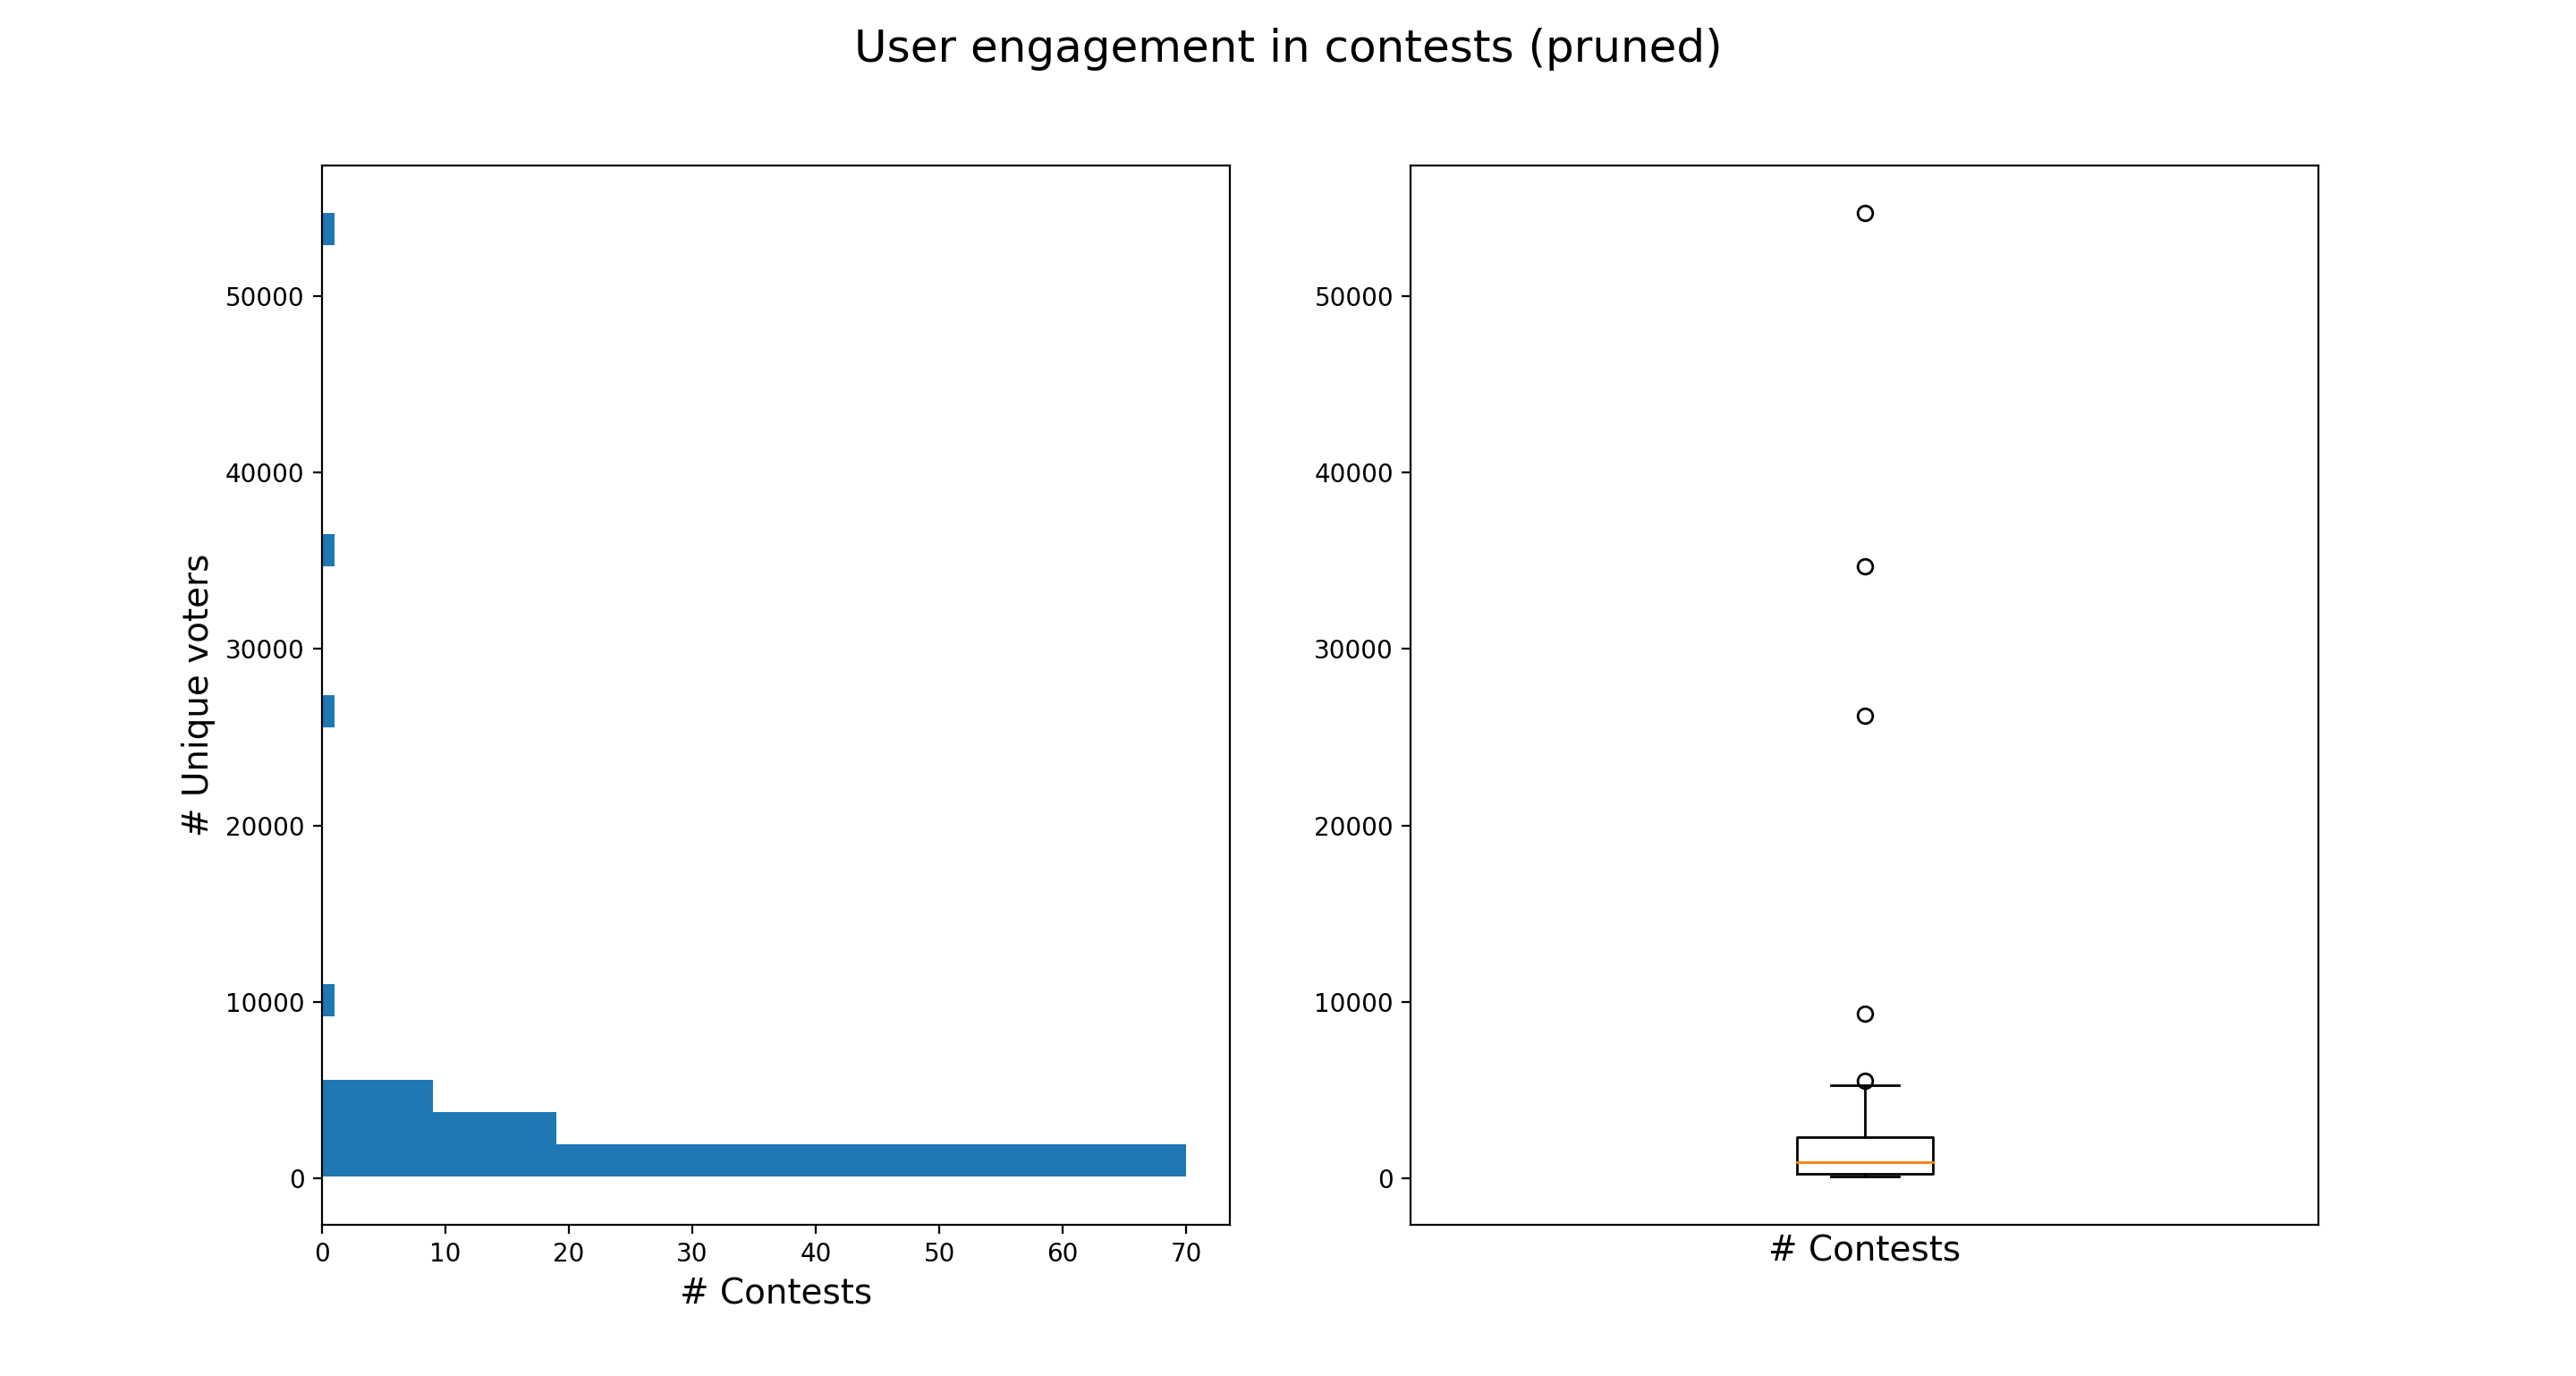
\includegraphics[width=1\textwidth]{Images/user_engagement_in_contests-pruned.png}
            \caption{The number of unique voters over contests after filtering out contests with less than 100 unique voters.}
            \label{user_engagement_in_contests-pruned}
        \end{center}
    \end{figure}
    
    The six large contests are worth investigating a bit more closely. Four \footnote{\url{https://choicely.com/contest/5ca98554-0f7d-11e7-9f0c-6f102a54d68d}}\footnote{\url{https://choicely.com/contest/fb112461-9000-11e6-9e28-87ebd7a21d0d}}\footnote{\url{https://choicely.com/contest/7425566e-8c8e-11e6-b8ce-2147b021362f}}\footnote{\url{https://choicely.com/contest/164f52c7-9df8-11e7-b3c9-d1a0f88250ad}}
    out of the six large contests were beauty pageants, labeled with the categories of "beauty", "fashion" and "entertainment". The two other contests\footnote{\url{https://choicely.com/contest/50819173-f838-11e6-b171-b949f18a4d21}}\footnote{\url{https://choicely.com/contest/4257ea9c-3e21-11e7-84ec-5f5a9bcfd190}}
    are listed only in the "other" category, which is certainly a mistake. By looking at the latter two contests, it can be easily seen that they would better belong to the "entertainment" and "sports" category. In each of the contests, the contest participants were people: either sportsmen, celebrities or beauty queens/kings. It is interesting that none of the large contests have had objects, places or other intangibles as contest participants, although the platform has seen many of such participants previously. 

    In the next step, let us look at the distribution of contest categories in the filtered set of contests. It can be seen from the histogram on Figure \ref{contests_over_categories}, that the amount of "beauty", "entertainment", "sport" and "fashion" contests is considerably high compared to the rest of the categories. This finding is well aligned with the case company's profile at the point of conducting this study. As pointed out in Chapter \ref{section::introduction-to-the-choicely-voting-platform}, most of the company's customer base consits of Finnish broadcasters and advertisers. Hence there is no surprise in the distribution of the categories except for the "other" group. 
    
    \begin{figure}[h] 
        \begin{center}
            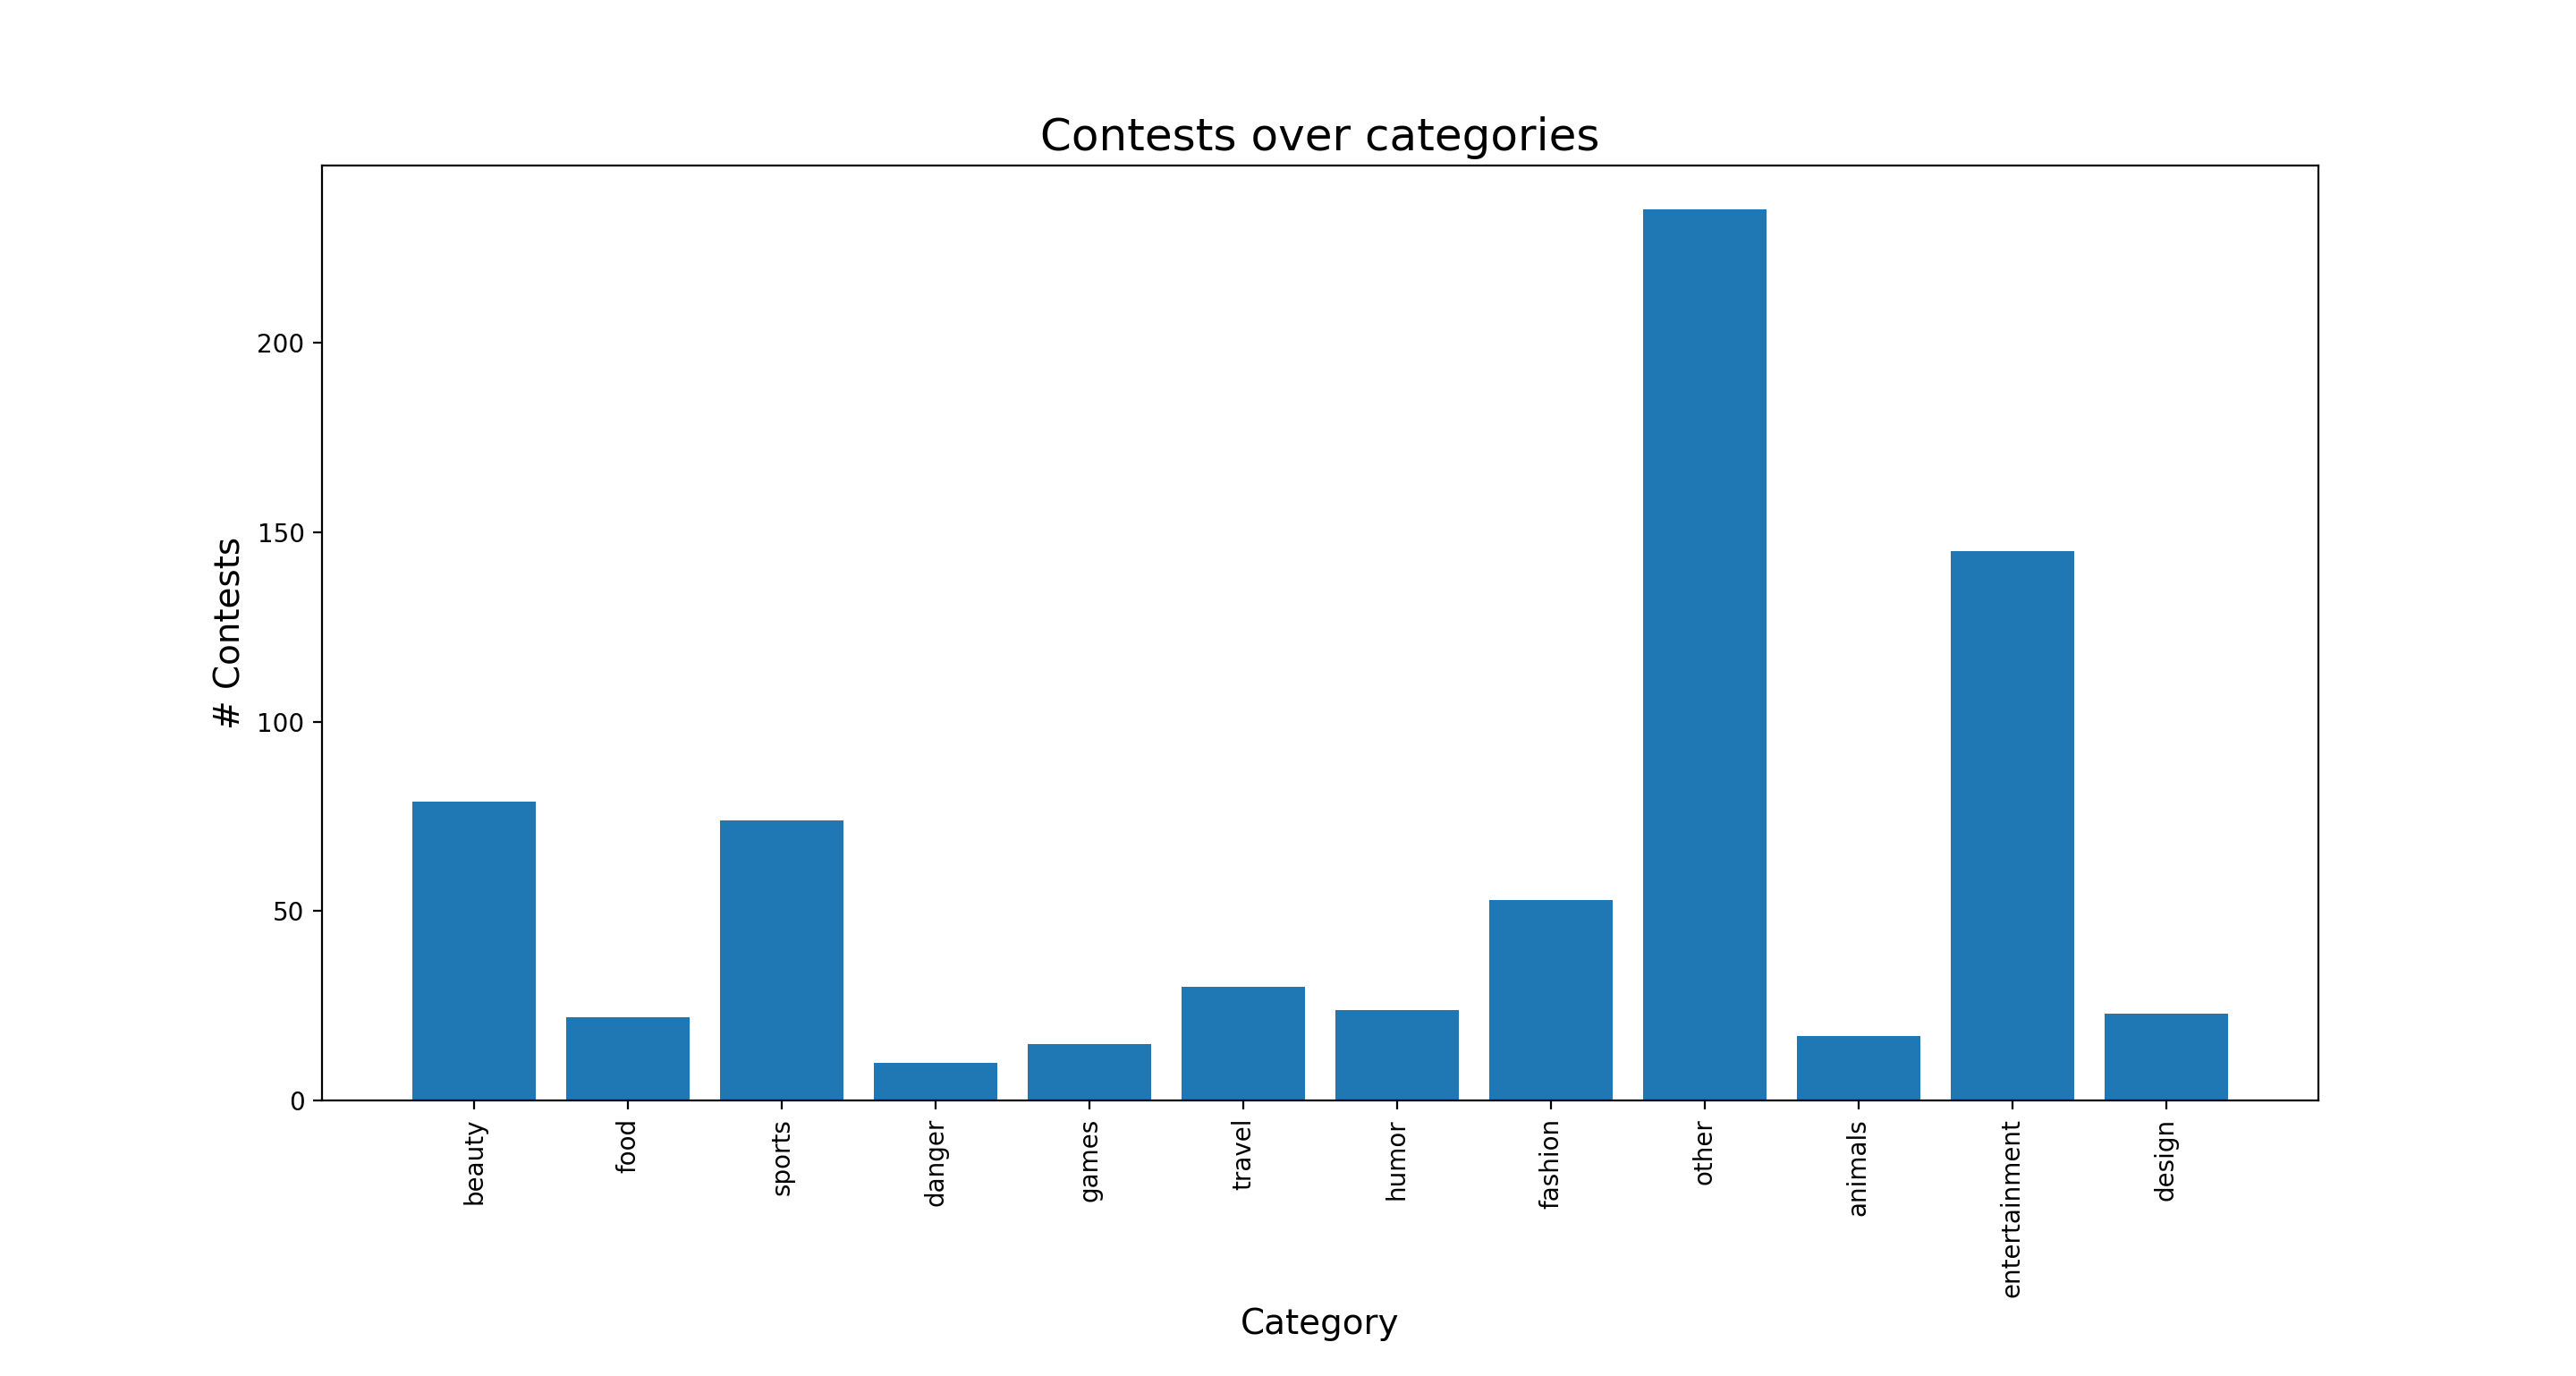
\includegraphics[width=1\textwidth]{Images/contests_over_categories.png}
            \caption{The number of contests in each category.}
            \label{contests_over_categories}
        \end{center}
    \end{figure}
    
    By manually looking at contests in the "other" category it can be seen, that many (28 out of 34) of these contests is actually a sport-related. To name a few examples, there are contests with titles as "Best player poll" ("Paras pelejaa aanestys")\footnote{\url{https://choicely.com/contest/5f8f8470-914d-11e6-bd5b-e571d894172f}}, "Who is the hottest driver?" ("Kuka on kuumin kuski?")\footnote{\url{https://choicely.com/contest/93d5f89c-5676-11e7-8cf7-0759c198269e}}, "Fastest driver of the race" ("Kisan nopein kuski")\footnote{\url{https://choicely.com/contest/bb7db707-3683-11e7-9f48-cbe34704f83e}}. This finding is not a suprise knowing the firm's customer base, but it also suggests the popularity of sports contests. If these contests were labeled correctly, sports contest would top the charts (Figure \ref{contests_over_categories}) with the highest bin around 50. Another interesting fact is, that in all of the sports contests, participants are athletes, hence the images contain human beings as well. 
    
    Moreover, three of the contests were related to the "travel" category, one to "fashion" and "beauty" and one to "entertainment". The error in this case is not as high as with sport contests, however correcting these category labels would facilitate data analysis in the future. For this reason, it is suggested to the company to review such issues, correct them manually and potentially prevent them happening in the future. 
    
    To answer the question of most engaging contest categories, the unique voters over contest categories is studied. Simple statistical measures (sum, mean, median and standard deviation) are calculated for the number of unique voters for each contest category. Table \ref{user_engagement_over_categories} displays the results.
    
    It can be seen, that "entertainment" and "beauty" contests cover the majority the amount of unique voters ($\approx 66.60 \%$ of the total). The values of these categories together are similar with the  "fashion" category. In these categories the mean and the median of the voters is also considerably high, which suggests their attractiveness. However, the high values in the standard deviation of the unique voters indicate that values are widely spread around the mean. The relevance of this observation is, that not all contests in these categories engage a large audience necessarily. Thus it can be concluded, that these categories tend to appear together and also attract a larger audience compared to the rest in general. 

    \begin{table}[]
        \centering
        \begin{adjustbox}{width=1\textwidth}
            \begin{tabular}{l|c|c|c|c|c}
                \textbf{Contest category} & \textbf{Sum of unique voters} & \textbf{Mean of unique voters} & \textbf{Median of unique voters} & \textbf{Standard deviation of unique voters} \\
                \hline
                beauty & 135866 & 3996.06 & 1482.00 & 9854.14 \\
                other & 61455 & 1807.50 & 1240.50 & 1831.40 \\
                entertainment & 161233 & 5374.43 & 1728.50 & 11772.68 \\
                sports & 15220 & 634.17 & 299.00 & 757.83 \\
                fashion & 75872 & 4742.00 & 874.00 & 12972.72 \\
                travel & 4451 & 1483.67 & 409.00 & 1719.40 \\
                humor & 1367 & 683.50 & 683.50 & 274.50 \\
                food & 767 & 767.00 & 767.00 & 0.00 \\
                danger & 958 & 958.00 & 958.00 & 0.00 \\
                games & 164 & 164.00 & 164.00 & 0.00
            \end{tabular}
        \end{adjustbox}
        \caption{The basic statistical measures of unique voters for each contest category.}
        \label{user_engagement_over_categories}
    \end{table}
    
    The categories "travel", "humor", "food", "danger" and "games" have hosted only a considerably low number of contests (Figure \ref{contests_over_categories}). Due to the small amount of data, it is difficult to derive any relevant results about the attractiveness of these categories at this point. It is suggested for the company to host and advertise more of these contests so that the public's opinion and engagement can be evaluated in these areas as well.

    % As the last part of the EDA, the attributes of highly rated contestants are investigated. In other words it is studied, what kind of traits make a contest participant more attractive to users. To answer this question, the podium finishers of the six large contests explained above are taken as examples. % TODO consider if needed

    % deriving results
    The above results contribute towards answering RQ2. The results allow to derive the following conclusions: 

    \begin{itemize}
        \item many of the contests are not labeled and hence belong only to the "other" category - fixing these labels manually could contribute towards better results,
        \item the "fashion", "beauty" and "entertainment" categories often appear together in contests,
        \item contests in the "beauty" and "entertainment" categories appear to be engaging to large audiences,
        \item contests where participants are human beings appear to be attractive to users,
        \item there is no correlation between the unique voter count and the number of participants,
        \item the platform has hosted only a few contests in some of the categories and hence it is not possible to derive significant findings about the attractiveness of those contest at the moment.
    \end{itemize}

\subsection{Association Analysis}
The results of the Association Analysis are presented in this chapter are limited to the 1-itemsets and 2-itemsets in order to keep the findings easily understandable. The following figures and paragraphs display and explain the results. The itemsets in the figures are ordered by the variance of the values over the bins (however the variances are not displayed in the figures). This way the itemset with the highest variance is on the top, while the itemset with the smallest variance is on the bottom of the figure. All of figures in this chapter follow this convention of ordering. First the chosen Miss Suomi 2017 contest is analyzed, followed by the system-level analysis.

% ---------------------------- BEGIN OF GENDER ANALYSIS ---------------------------- 
% \subsubsection{Single-item itemsets}
Figure \ref{itemset_supports-gender-Miss_Helsinki-1_itemset} displays the 1-itemset supports and lifts for genders. The first finding to note is the \emph{\{"beauty"\}} and \emph{\{"dress"\}} itemsets with support and lift values 1.0 for all genders on the bottom of the figures. These values suggest that every single vote transaction in this contest has contained these itemsets. The reason behind this observation is that all of the participants' images had these labels. Therefore, inevitably all of the vote transactions picked up these itemsets and every vote in the contest has full support towards them. Such values do not show any significant meaning and therefore are excluded from the rest of the figures.

\begin{figure}[]
    \begin{center}
        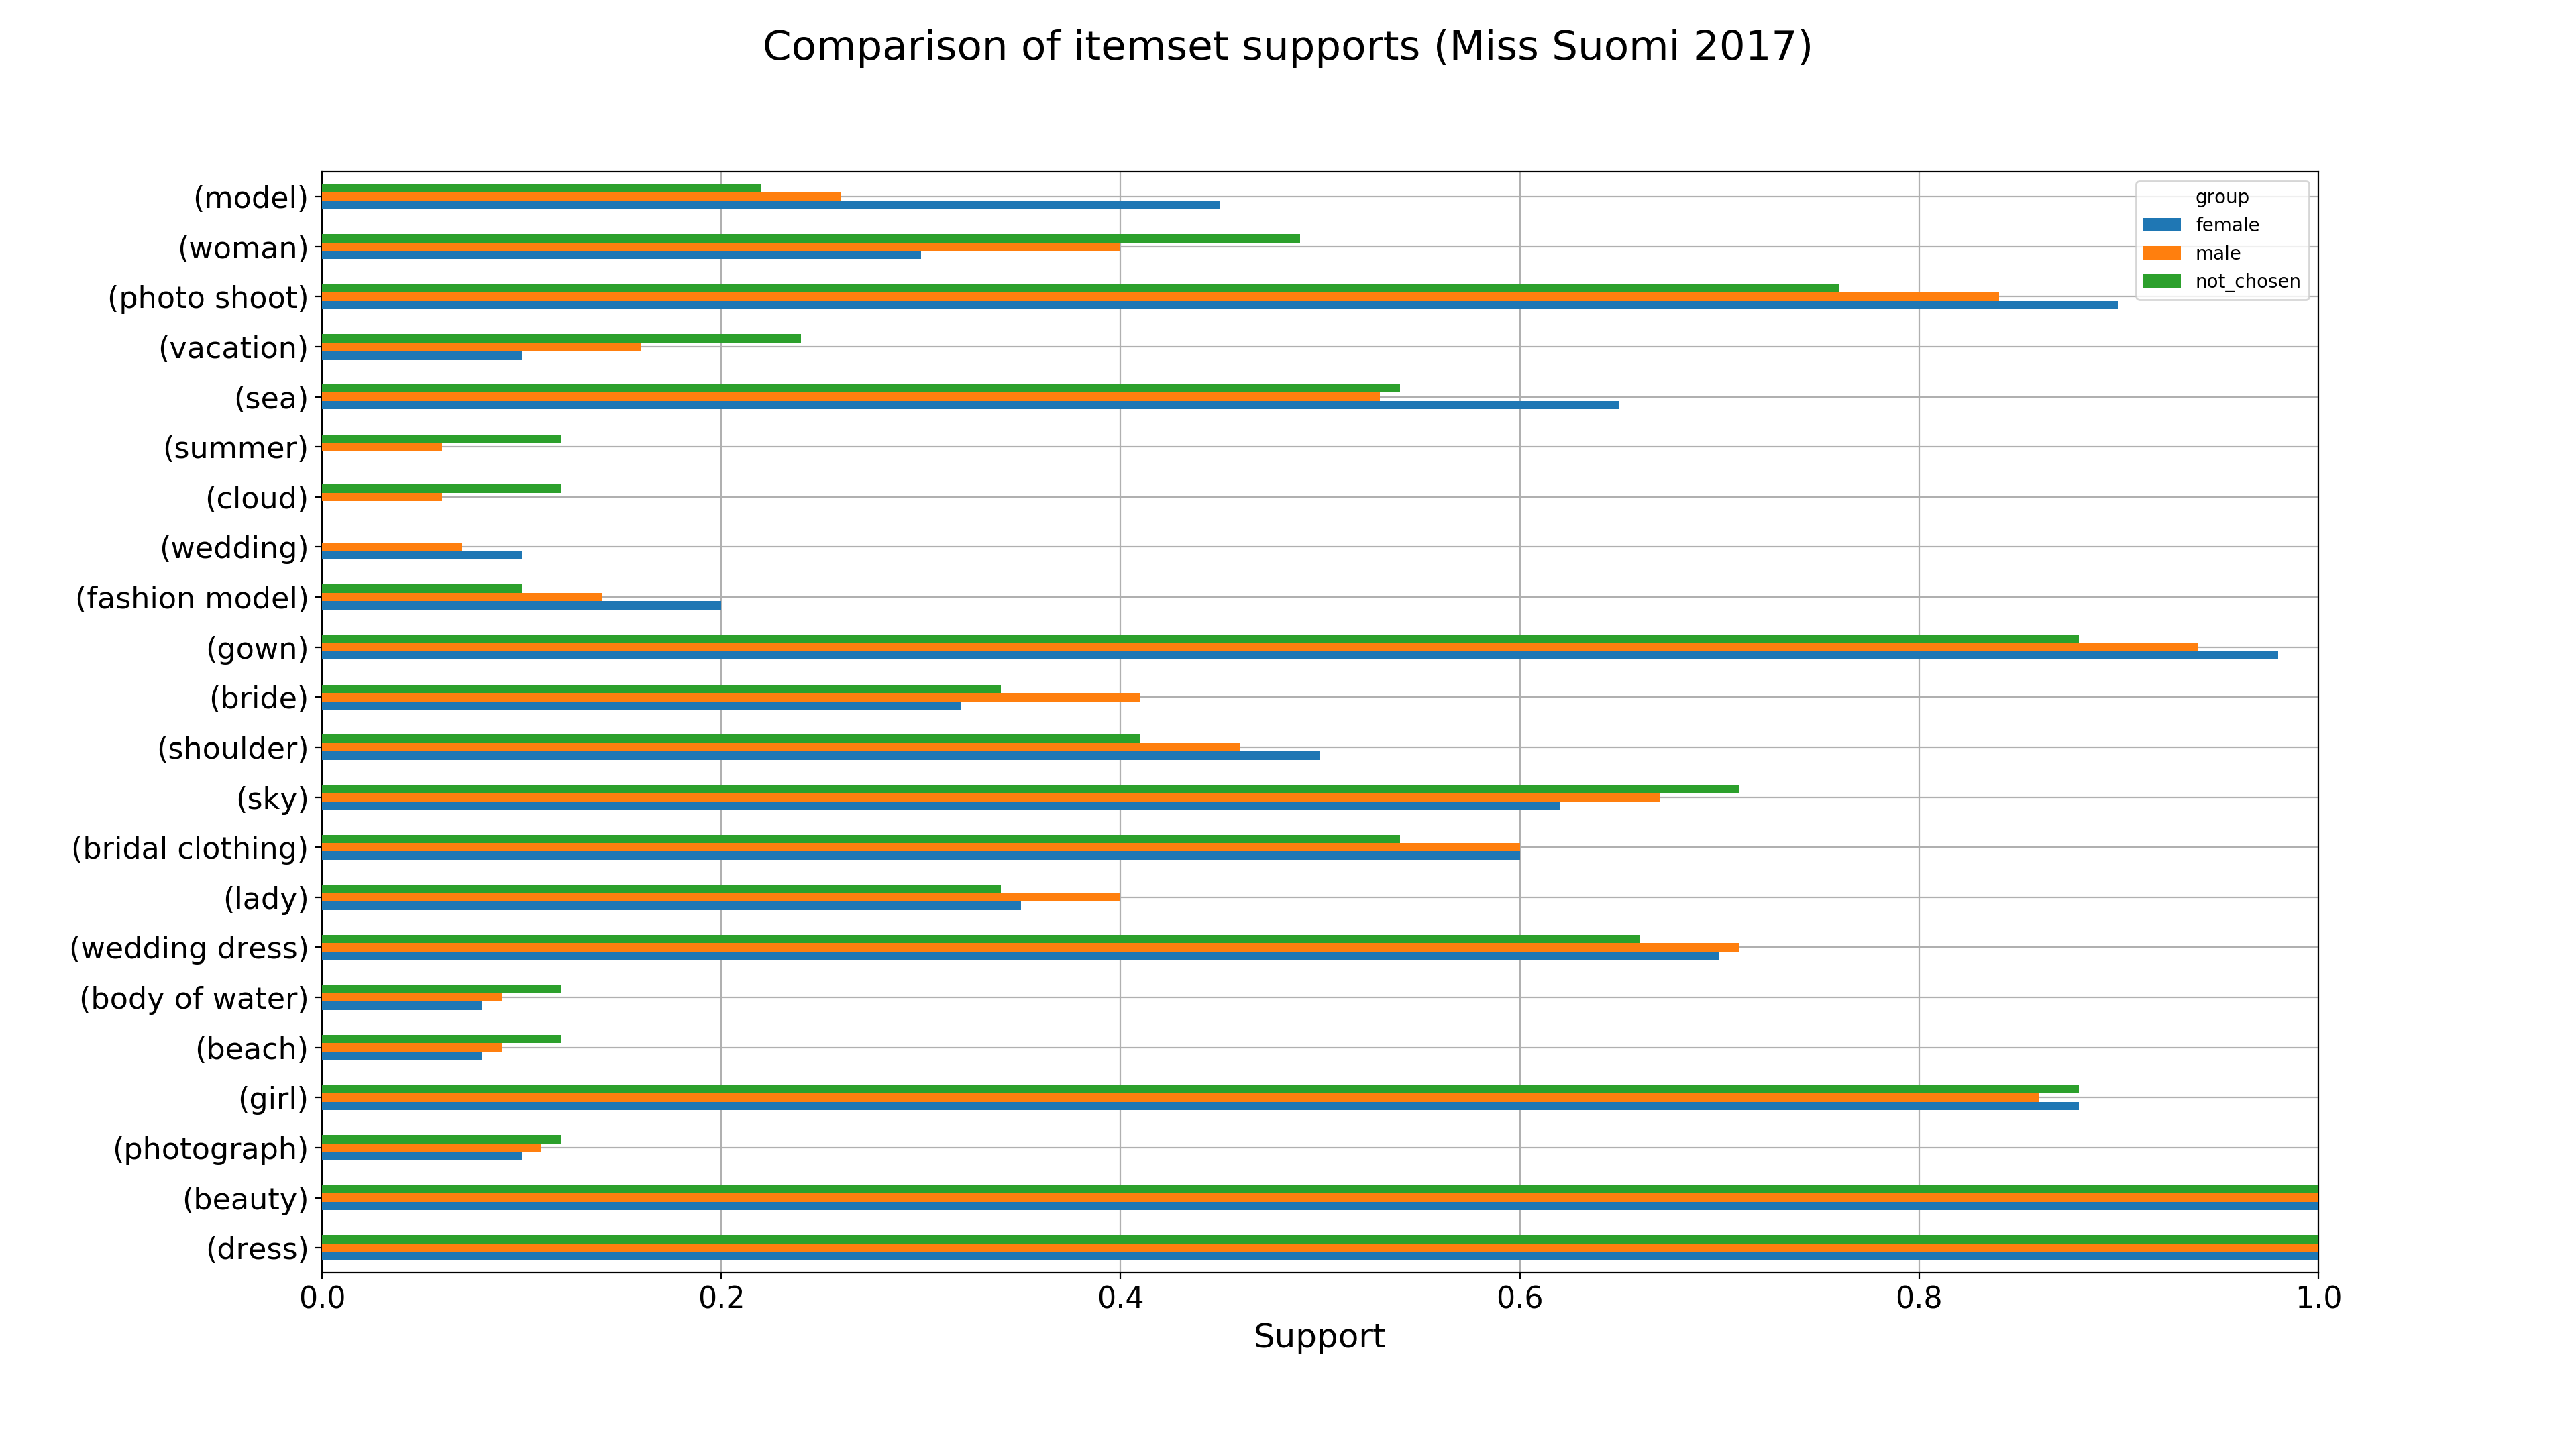
\includegraphics[width=1.2\textwidth,center]{Images/itemset_supports-gender-Miss_Helsinki-1_itemset.png}
        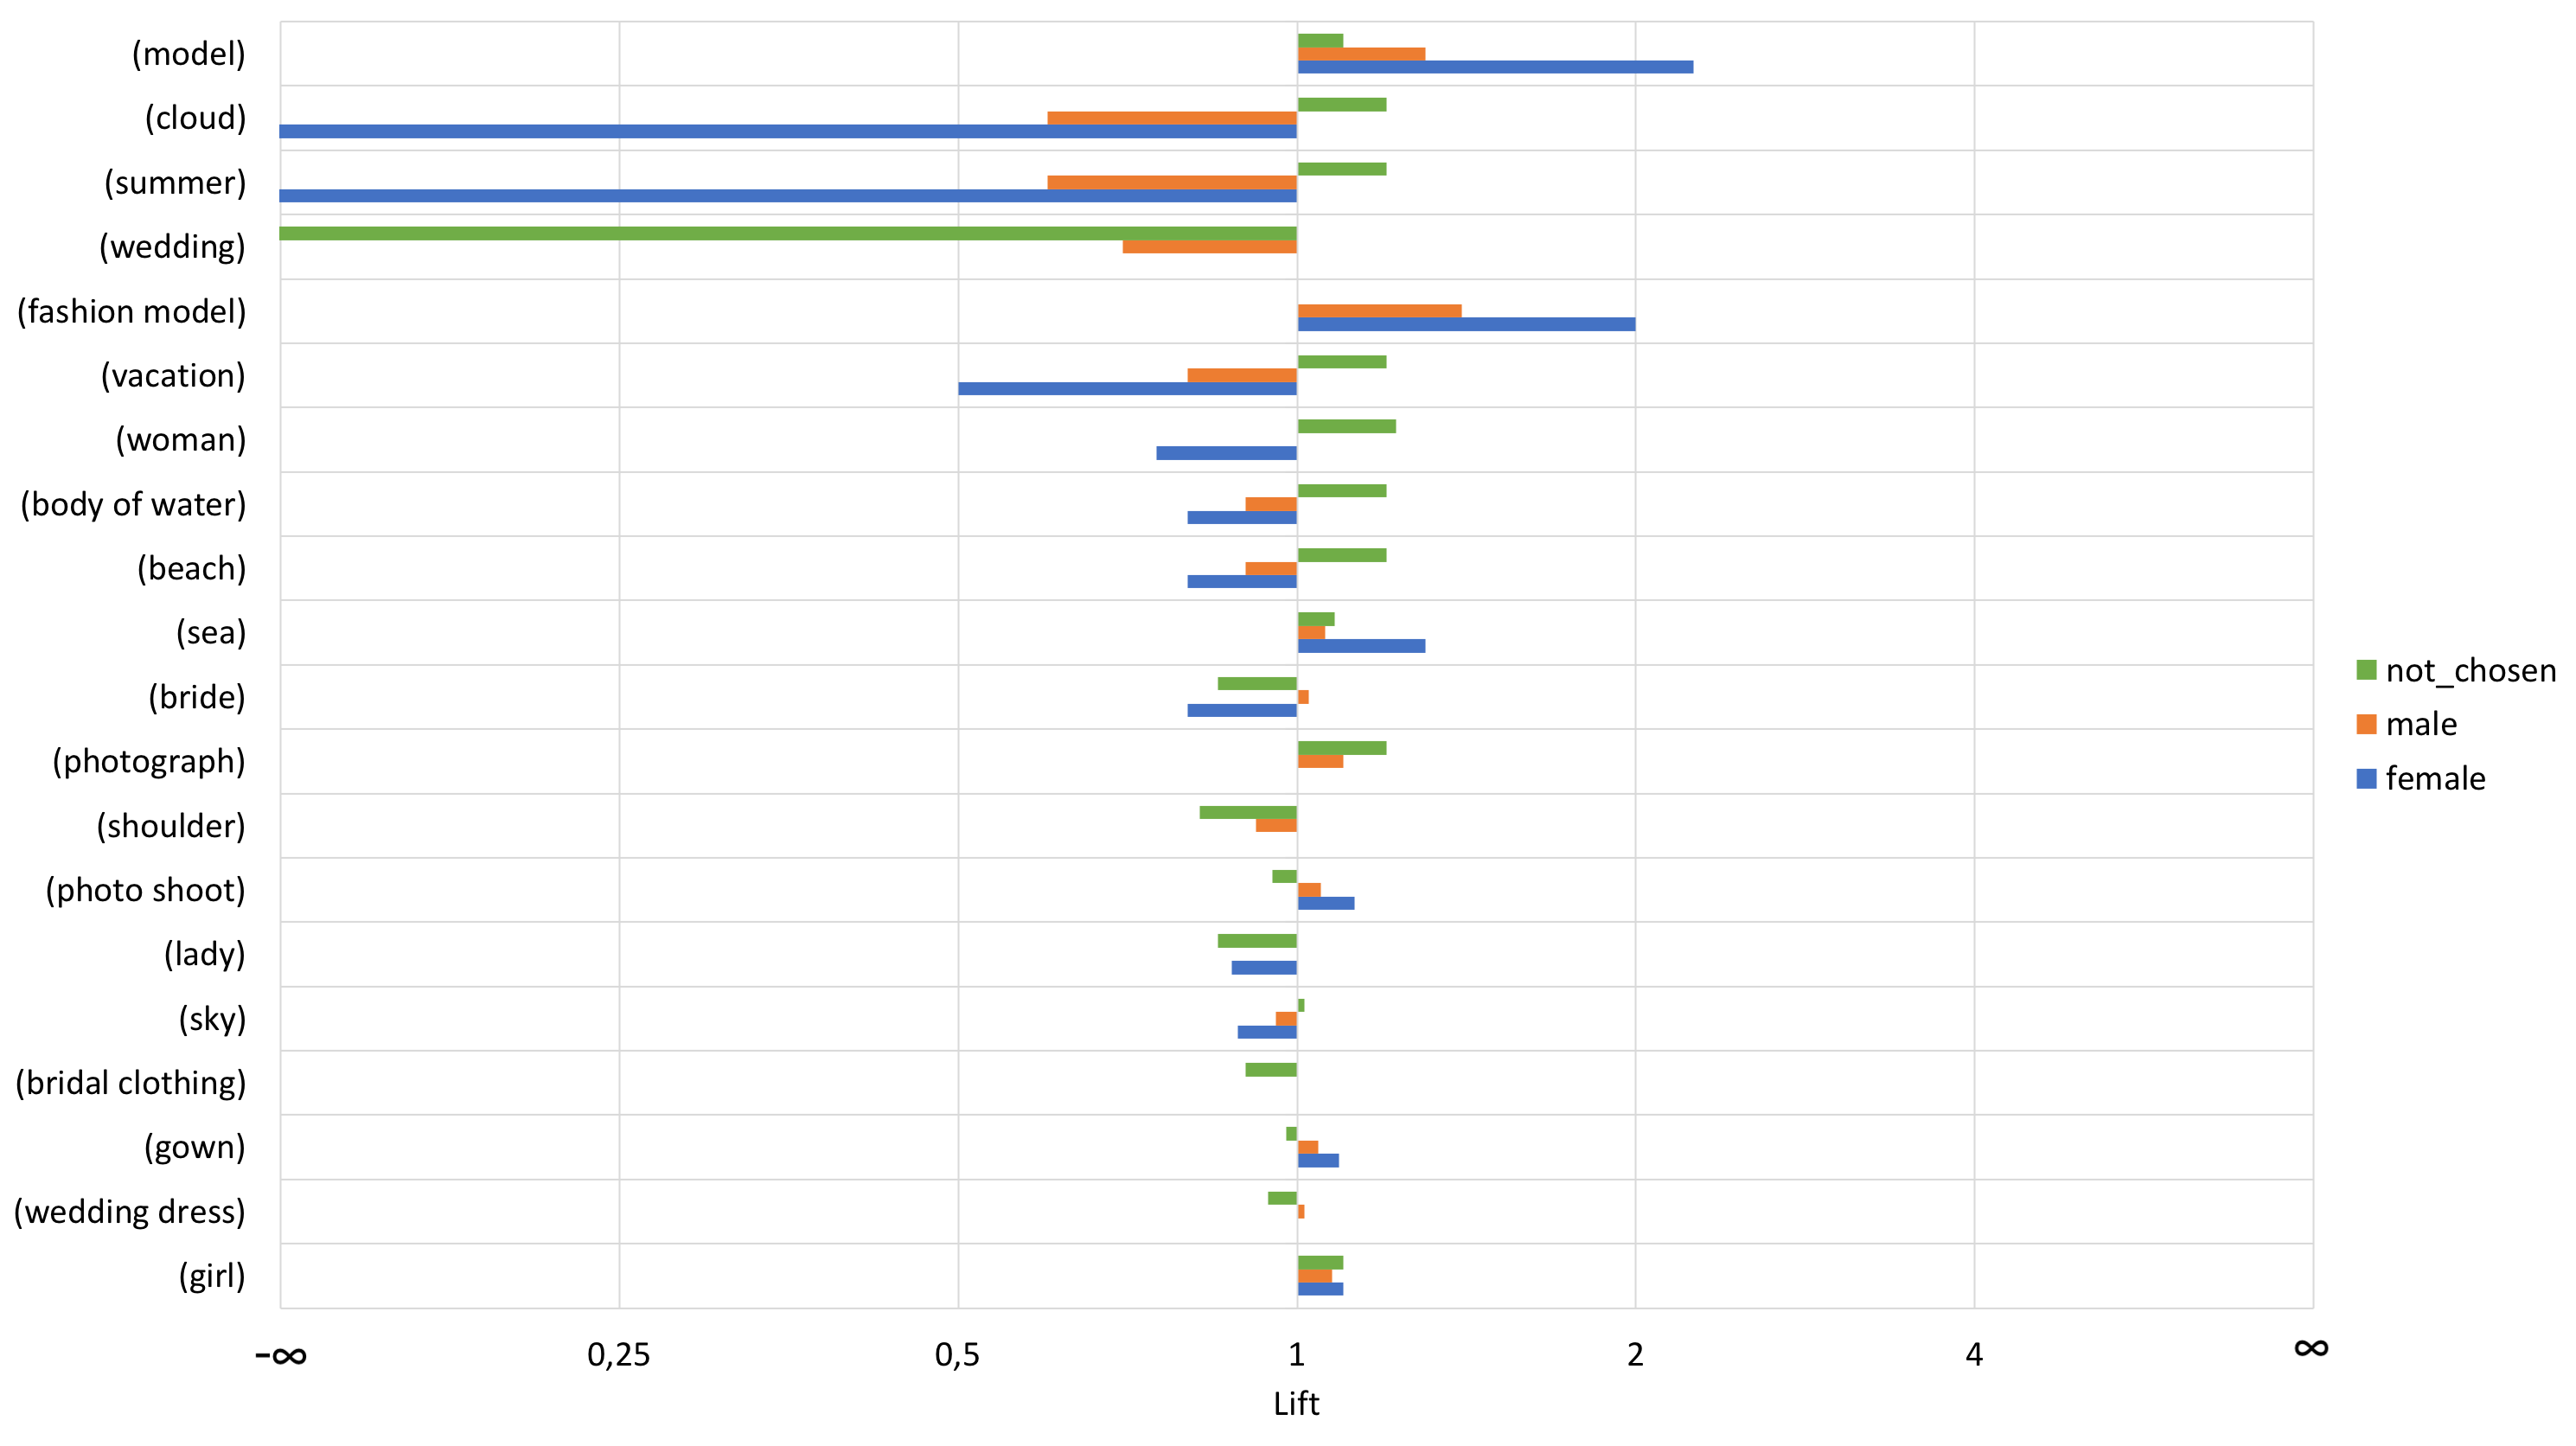
\includegraphics[width=1.2\textwidth,center]{Images/itemset_lifts-gender-Miss_Suomi-1_itemsets.png}
        \caption{The 1-itemset supports (top) and lifts (bottom) in the Miss Suomi 2017 contest by genders (all itemsets are displayed ordered by the variance of the values).}
        \label{itemset_supports-gender-Miss_Helsinki-1_itemset}
    \end{center}
\end{figure}

It is interesting to investigate, why all of the images contained these two labels in general. As the participants' images were shot in a similar environment, with considerably similar content (e.g. the white dresses, the background, the hair styles, only one model in the image etc.), the Google Vision API assigned the same labels to the images. This gives a proof that computer vision in this case is more targeted towards getting an overall idea about the content of an image, rather than identifying its specific traits and attributes. 

Figure \ref{itemset_supports-age_group-Miss_Helsinki-1_itemset} provides a good possibility also to compare gender differences. For instance, the support \emph{S(X=\{"model"\}|gender=female)=0.45} is considerably high than its male counterpart \emph{S(X=\{"model"\}|gender=male) = 0.26}. The lift values in this instance are \emph{L(X=\{"model"\}|gender=female) = 2.25} and \emph{L(X=\{"model"\}|gender = male) = 1.30}. Similar observation can be made for the \emph{\{"fashion model"\}} itemset, which suggests correlation between these two labels. This suggests two findings: the label "(fashion) model" appears to be more attractive to female voters compared to males and the presence of model in an image makes participants more appealing to all genders, but especially females. 

Similarly, the \emph{\{"photo shoot\}, \{"sea"\}, \{"gown"\}} and \emph{\{"wedding"\}} itemsets have higher support in case of female voters. This may suggest that females are more likely to vote on images, where the object (the model and the dress) is put more into focus. The lift values however reveal, that the interest for \emph{\{"sea"\}, \{"gown"\}} and \emph{\{"photo shoot\}} higher for all groups, which proposes the presence of sea in the background increases the number of votes. 

Another curious thing to note is the lift values of the \emph{\{"summer", "cloud", "beach"\}} itemsets, which are lower than 1.0 for both males and females. This observarion may suggest that having these in the background of the image is less attractive compared to the sea as background. Furthermore, \emph{\{"wedding"\}} has lift value less than 1.0 for genders other than females, which suggests less interest for this topic.  

Interestingly, the support and the lift for the \emph{\{"cloud"\}} and \emph{\{"summer"\}} itemsets are 0.0 for females, while the values of the male group are slightly higher. This means that no female users have voted on images with these labels (unless they belong to the \emph{not\_chosen} gender). This allows the conclusion that males might prefer images with more light and more colorful background in their votes. The lift and the support for \emph{\{"bride"\}} and \emph{\{"lady"\}} itemsets for males are also higher, which can mean that the model being a girl has more impact on their votes than her dress or the surroundings. However, as the lift value is not topping the charts for these itemsets, which suggests no major impact in users' behavior.

% ---------------------------- END OF GENDER ANALYSIS ---------------------------- 
% ---------------------------- BEGIN OF AGE GROUP ANALYSIS ---------------------------- 

Next, the 1-itemsets are calculated similarly in the same contest for age groups. Figure \ref{itemset_supports-age_group-Miss_Helsinki-1_itemset} displays results. It is interesting to notice that age groups 45-54 and 65+ have considerably higher support than the rest of the groups in case of the \emph{\{"shoulder"\}, \{"bridal clothing"\}} and the \emph{\{"wedding dress"\}} itemsets. The higher lift values for these itemsets are also higher for these groups which suggests its attractivenexx. It seems, that the open-sholder wedding dresses displayed on the pictures raise the engagement of these groups. This may indicate also that dresses become influential in favoring a model in this kind of a contest for these groups. In other words, dress may be a more important aspect than the model herself.

\begin{figure}[] 
    \begin{center}
        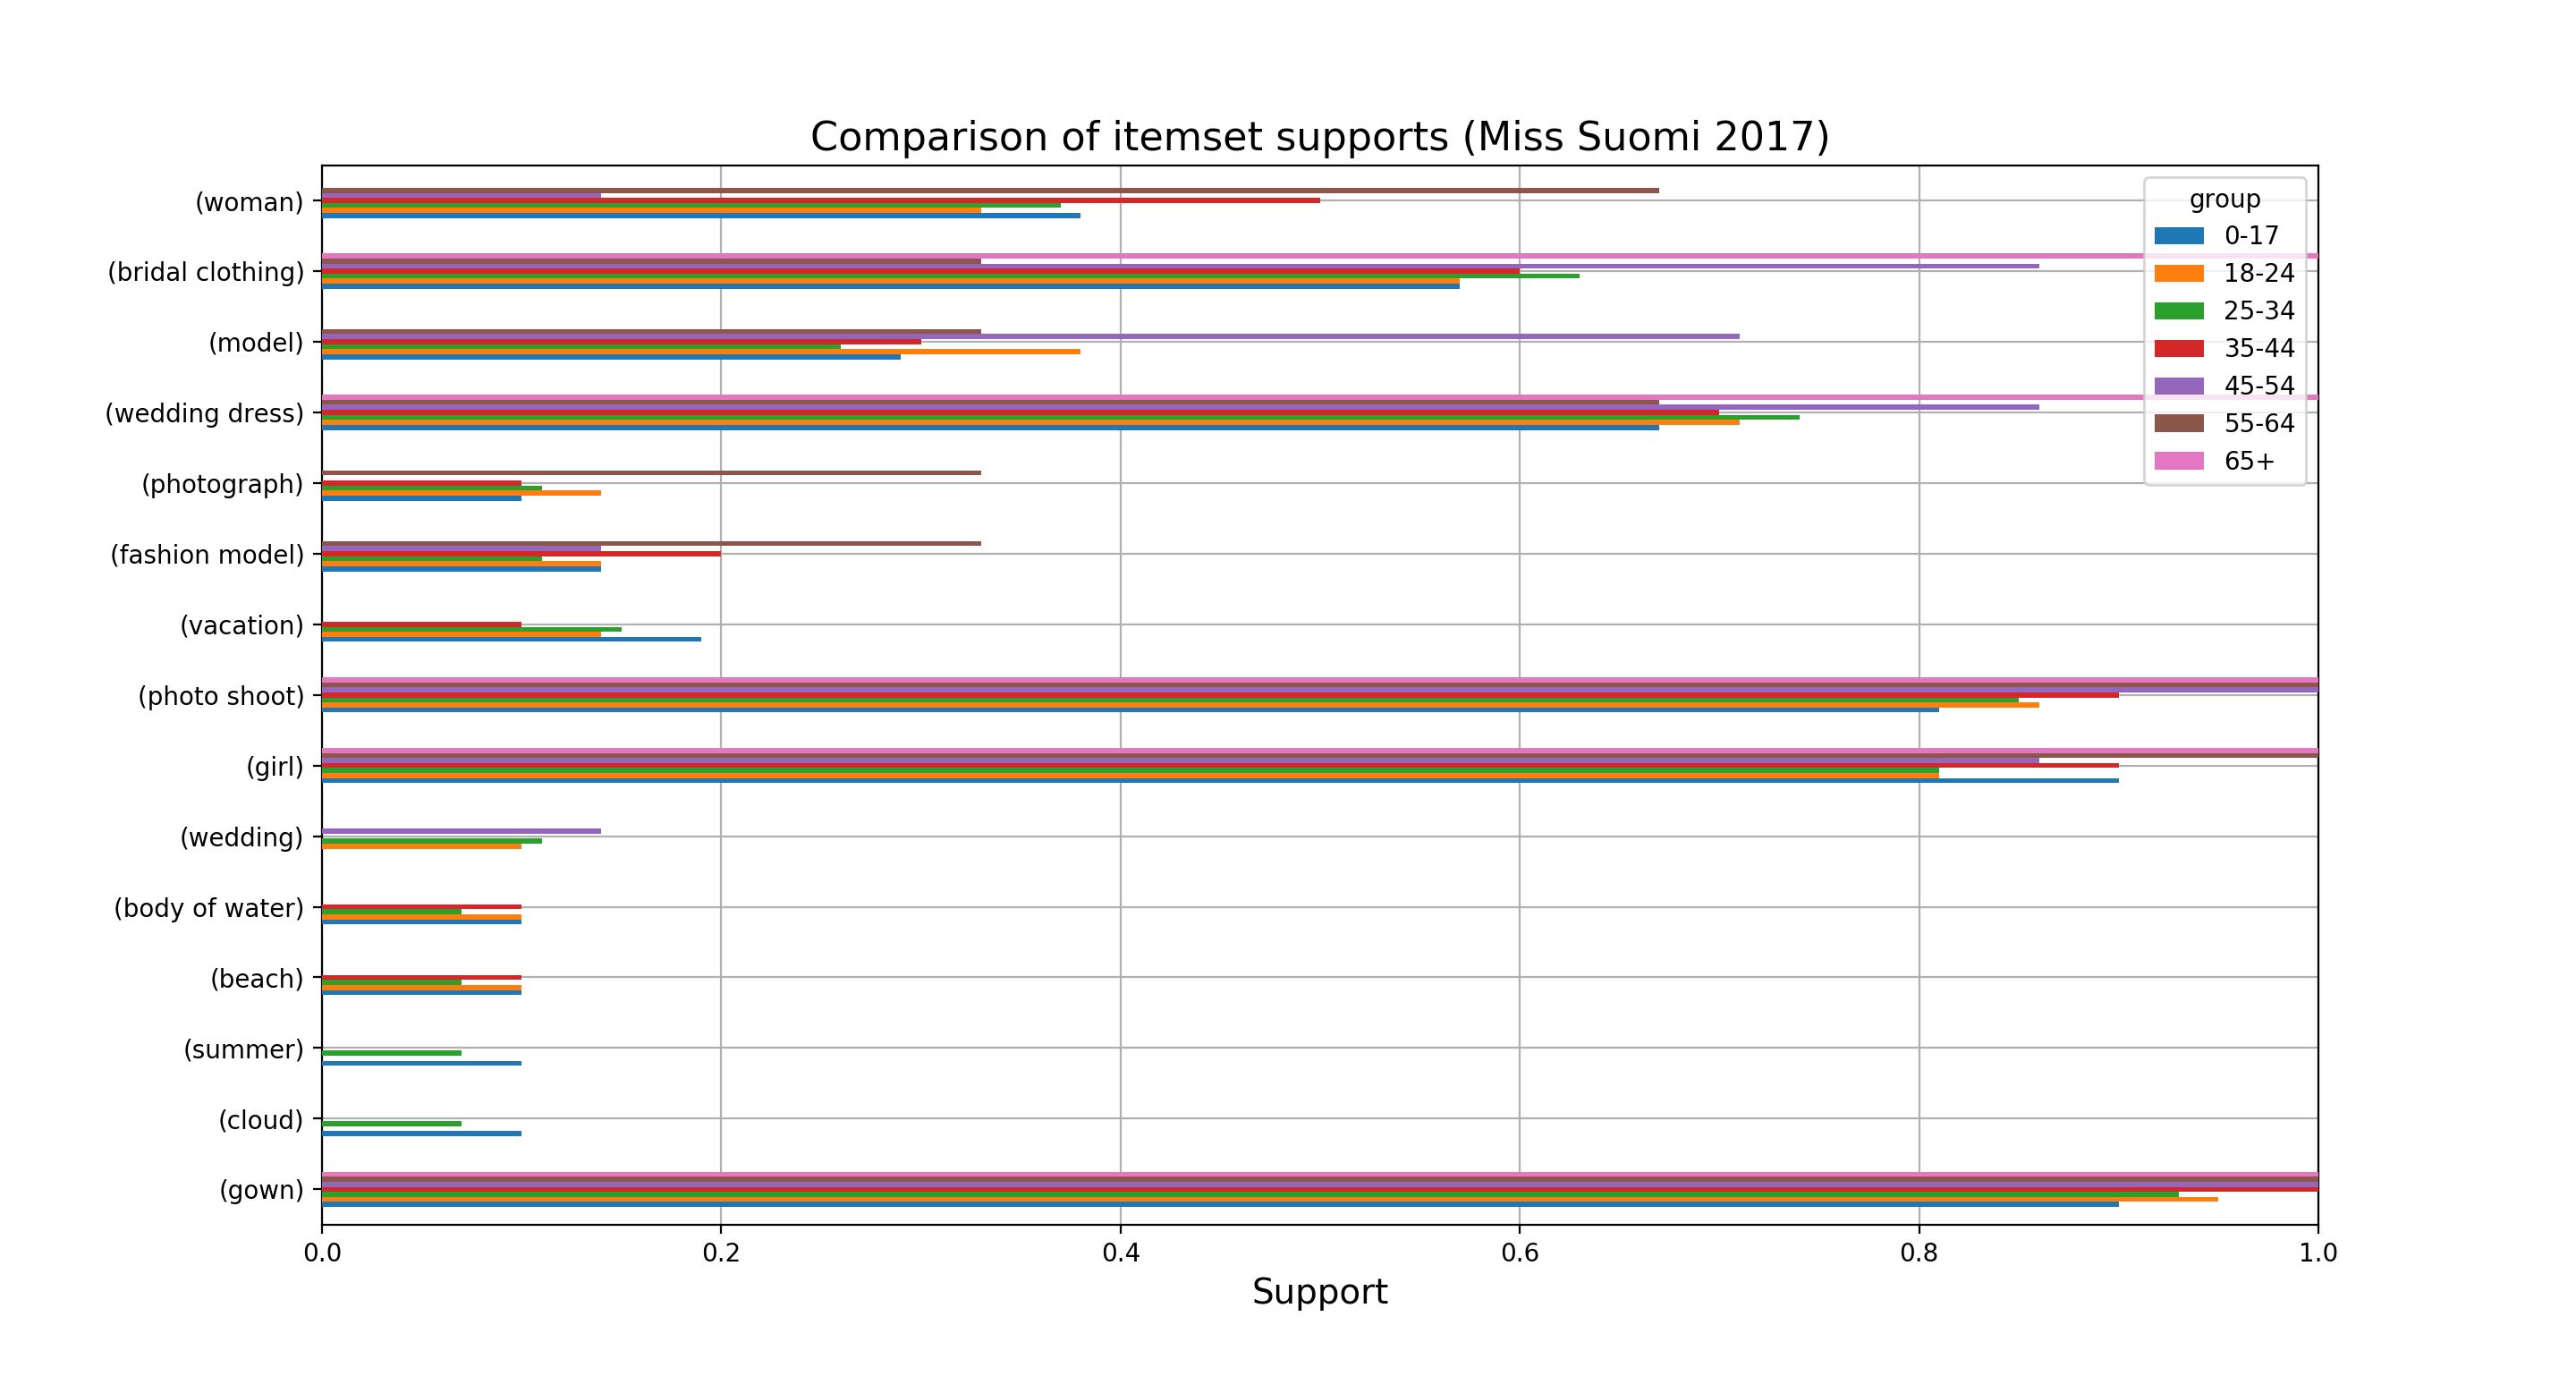
\includegraphics[width=1.2\textwidth,center]{Images/itemset_supports-age_group-Miss_Helsinki-1_itemset.png}
        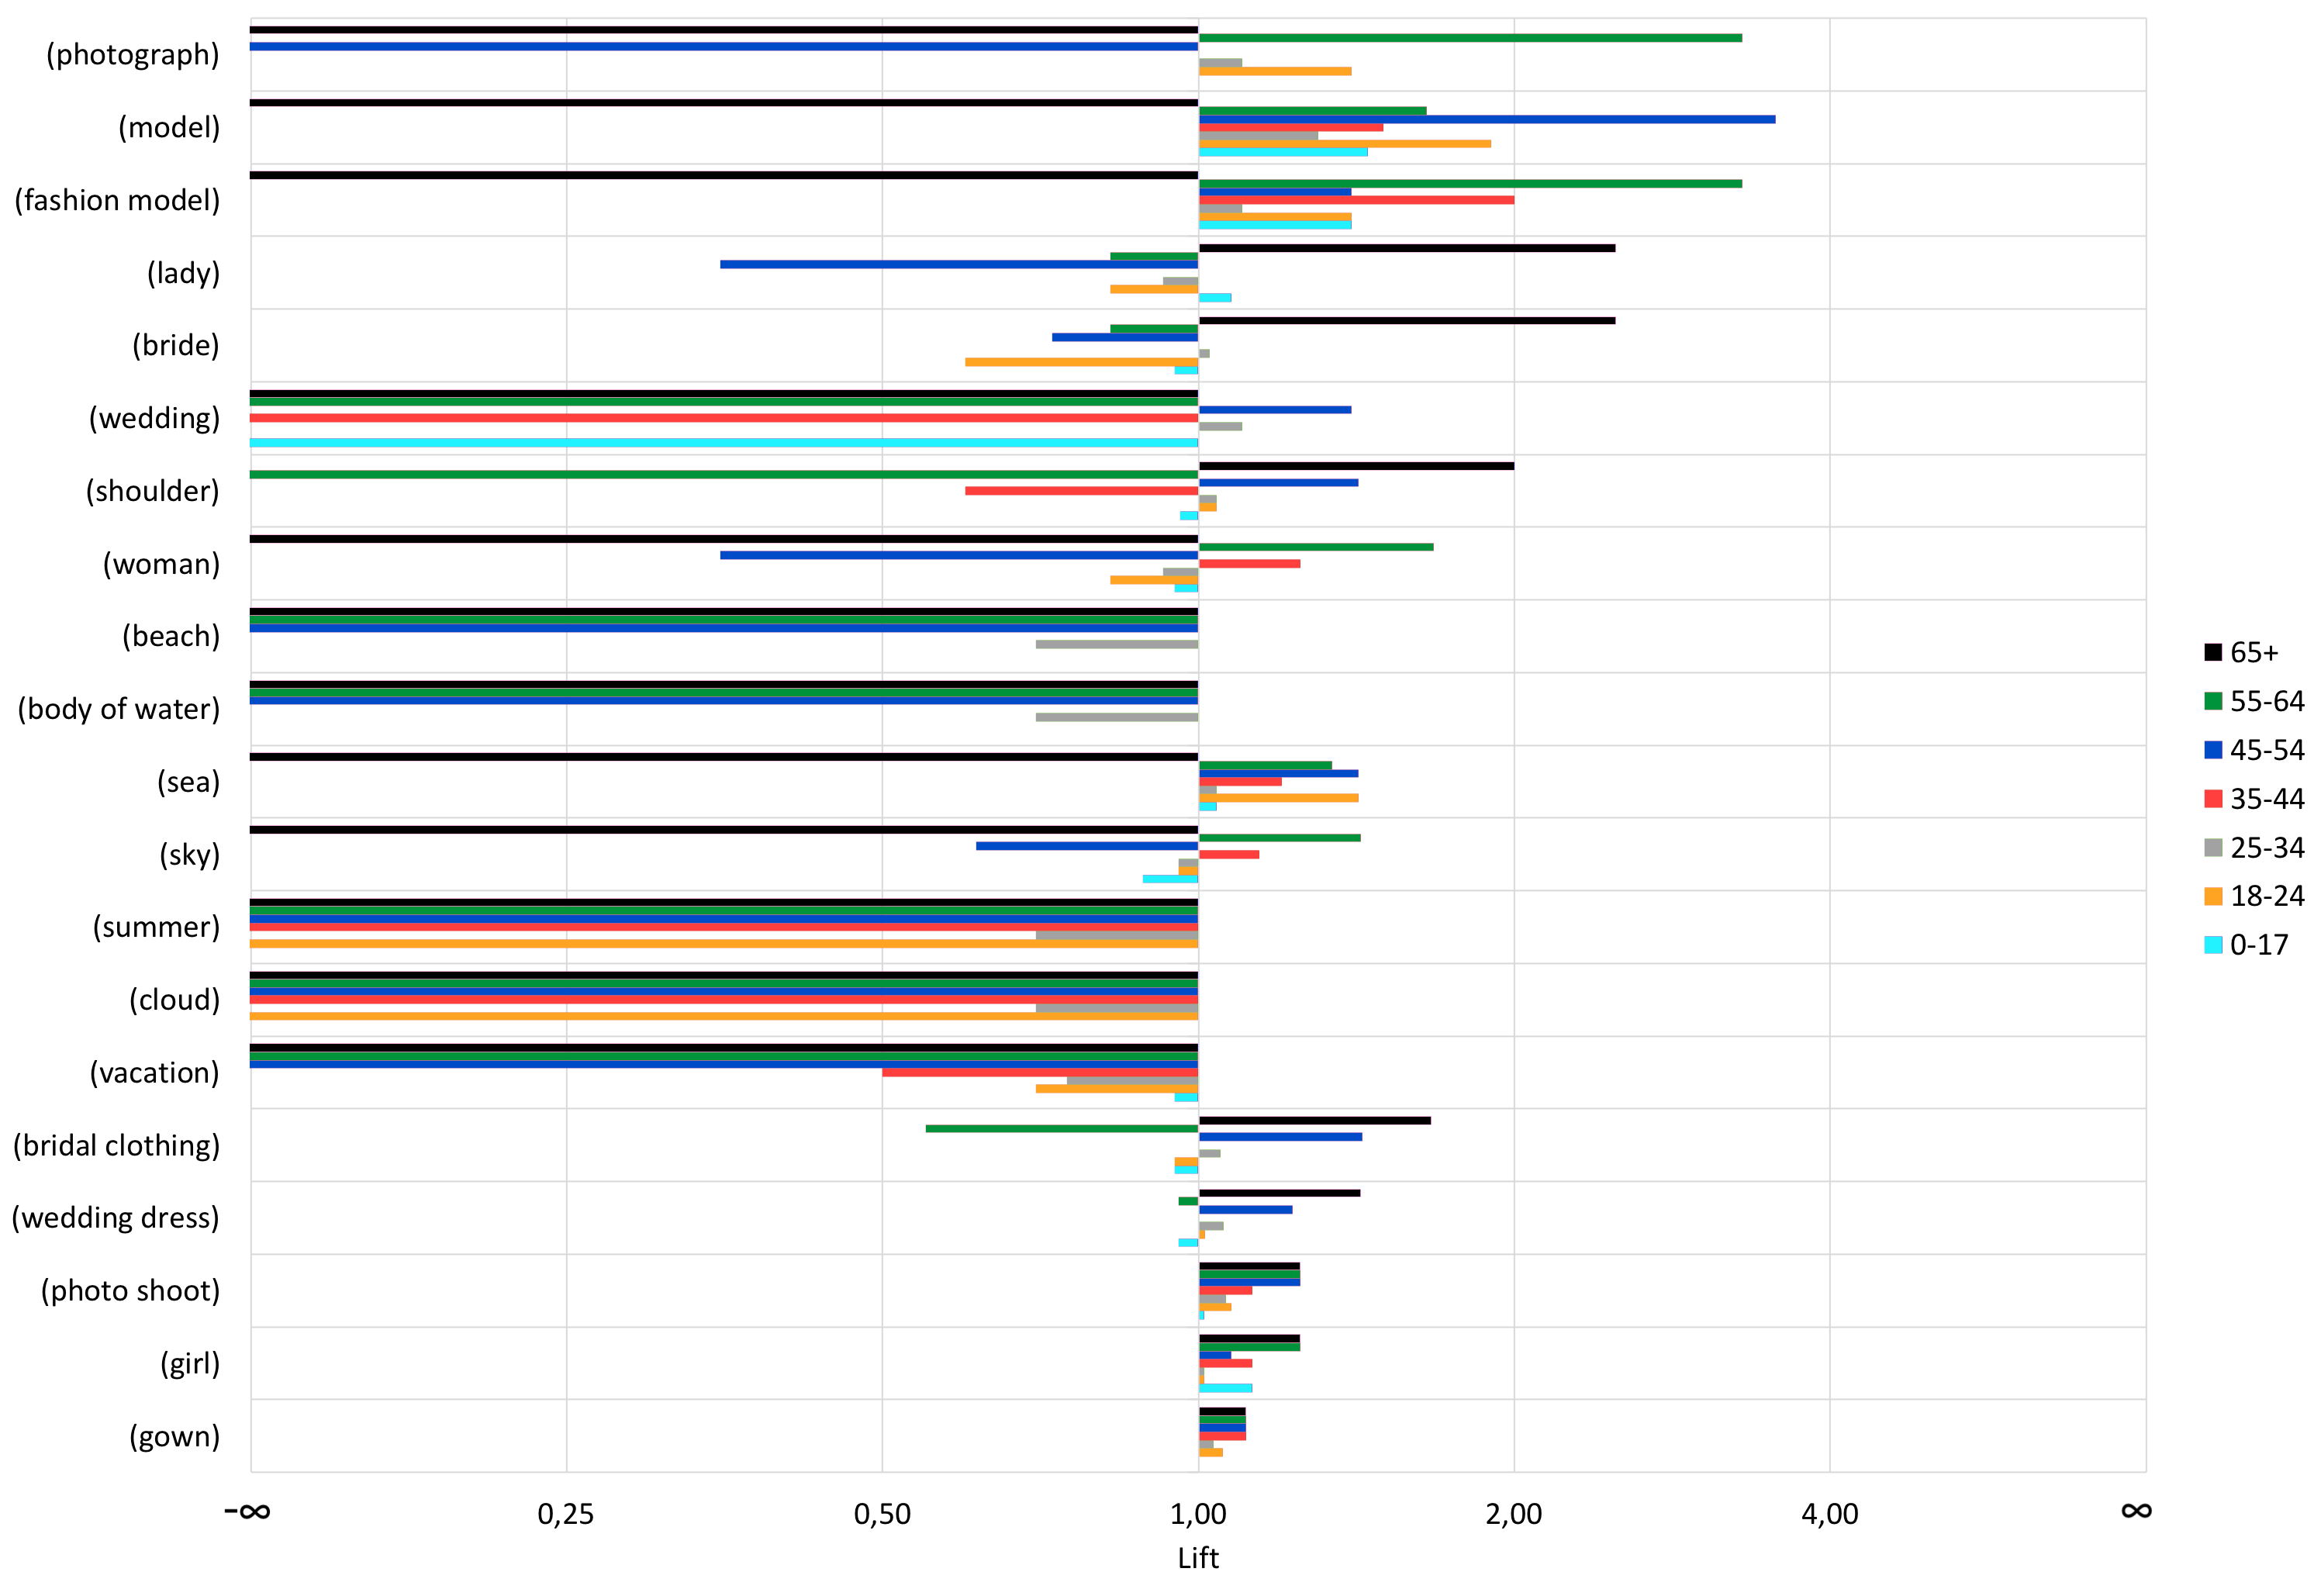
\includegraphics[width=1.2\textwidth,center]{Images/itemset_lifts-age_group-Miss_Suomi-1_itemsets.png}
        \caption{The 1-itemset supports (top) and lifts (bottom) in the Miss Suomi 2017 contest by age groups (only the first 15 itemsets are displayed ordered by the variance of the values).}
        \label{itemset_supports-age_group-Miss_Helsinki-1_itemset}
    \end{center}
\end{figure}

Another interesting observation is that the values for some itemsets, such as \emph{\{"body of water"\}, \{"beach"\}, \{"cloud"\}, \{"vacation"\}, \{"beach"\}} show 0.0 support and lift for the groups above age of 45. At the same time, these itemsets show somewhat higher support and lift by the rest of the age groups (0-17, 18-24, 25-34, 35-44). This finding may indicate that activities such as having vacation on a beach in a warm country is more in the interest of young people, which can be valuable information for travel agencies or marketing specialists. With such valuable information at hand, tourism offices could provide more customized advisory service for customers with different background. 

Strong difference can be observed in the lift values of \emph{\{"sea"\}} for the 65+ age group. The lift value is 0.0 in this case, while all the other groups have values over 1.0. This means that sea, as such did not engage the elderly whatsoever, while triggered the interest the rest of the groups. It can be hence said in general, that sea appears to be an attractive trait in the background for most of the age groups but does not interest voters above 65 years of age. 

% ---------------------------- END OF AGE GROUP ANALYSIS ---------------------------- 
% ---------------------------- BEGIN OF COUNTRY ANALYSIS ---------------------------- 

Finally, the 1-itemsets supports in the contest are analyzed by the location (country) of the users (Figure \ref{itemset_supports-country-Miss_Helsinki-1_itemset}). The first interesting observation is, that the support and lift of the USA group are 1.0 on some itemsets, while 0.0 on the others and there are no values in between. 

\begin{figure}[] 
    \begin{center}
        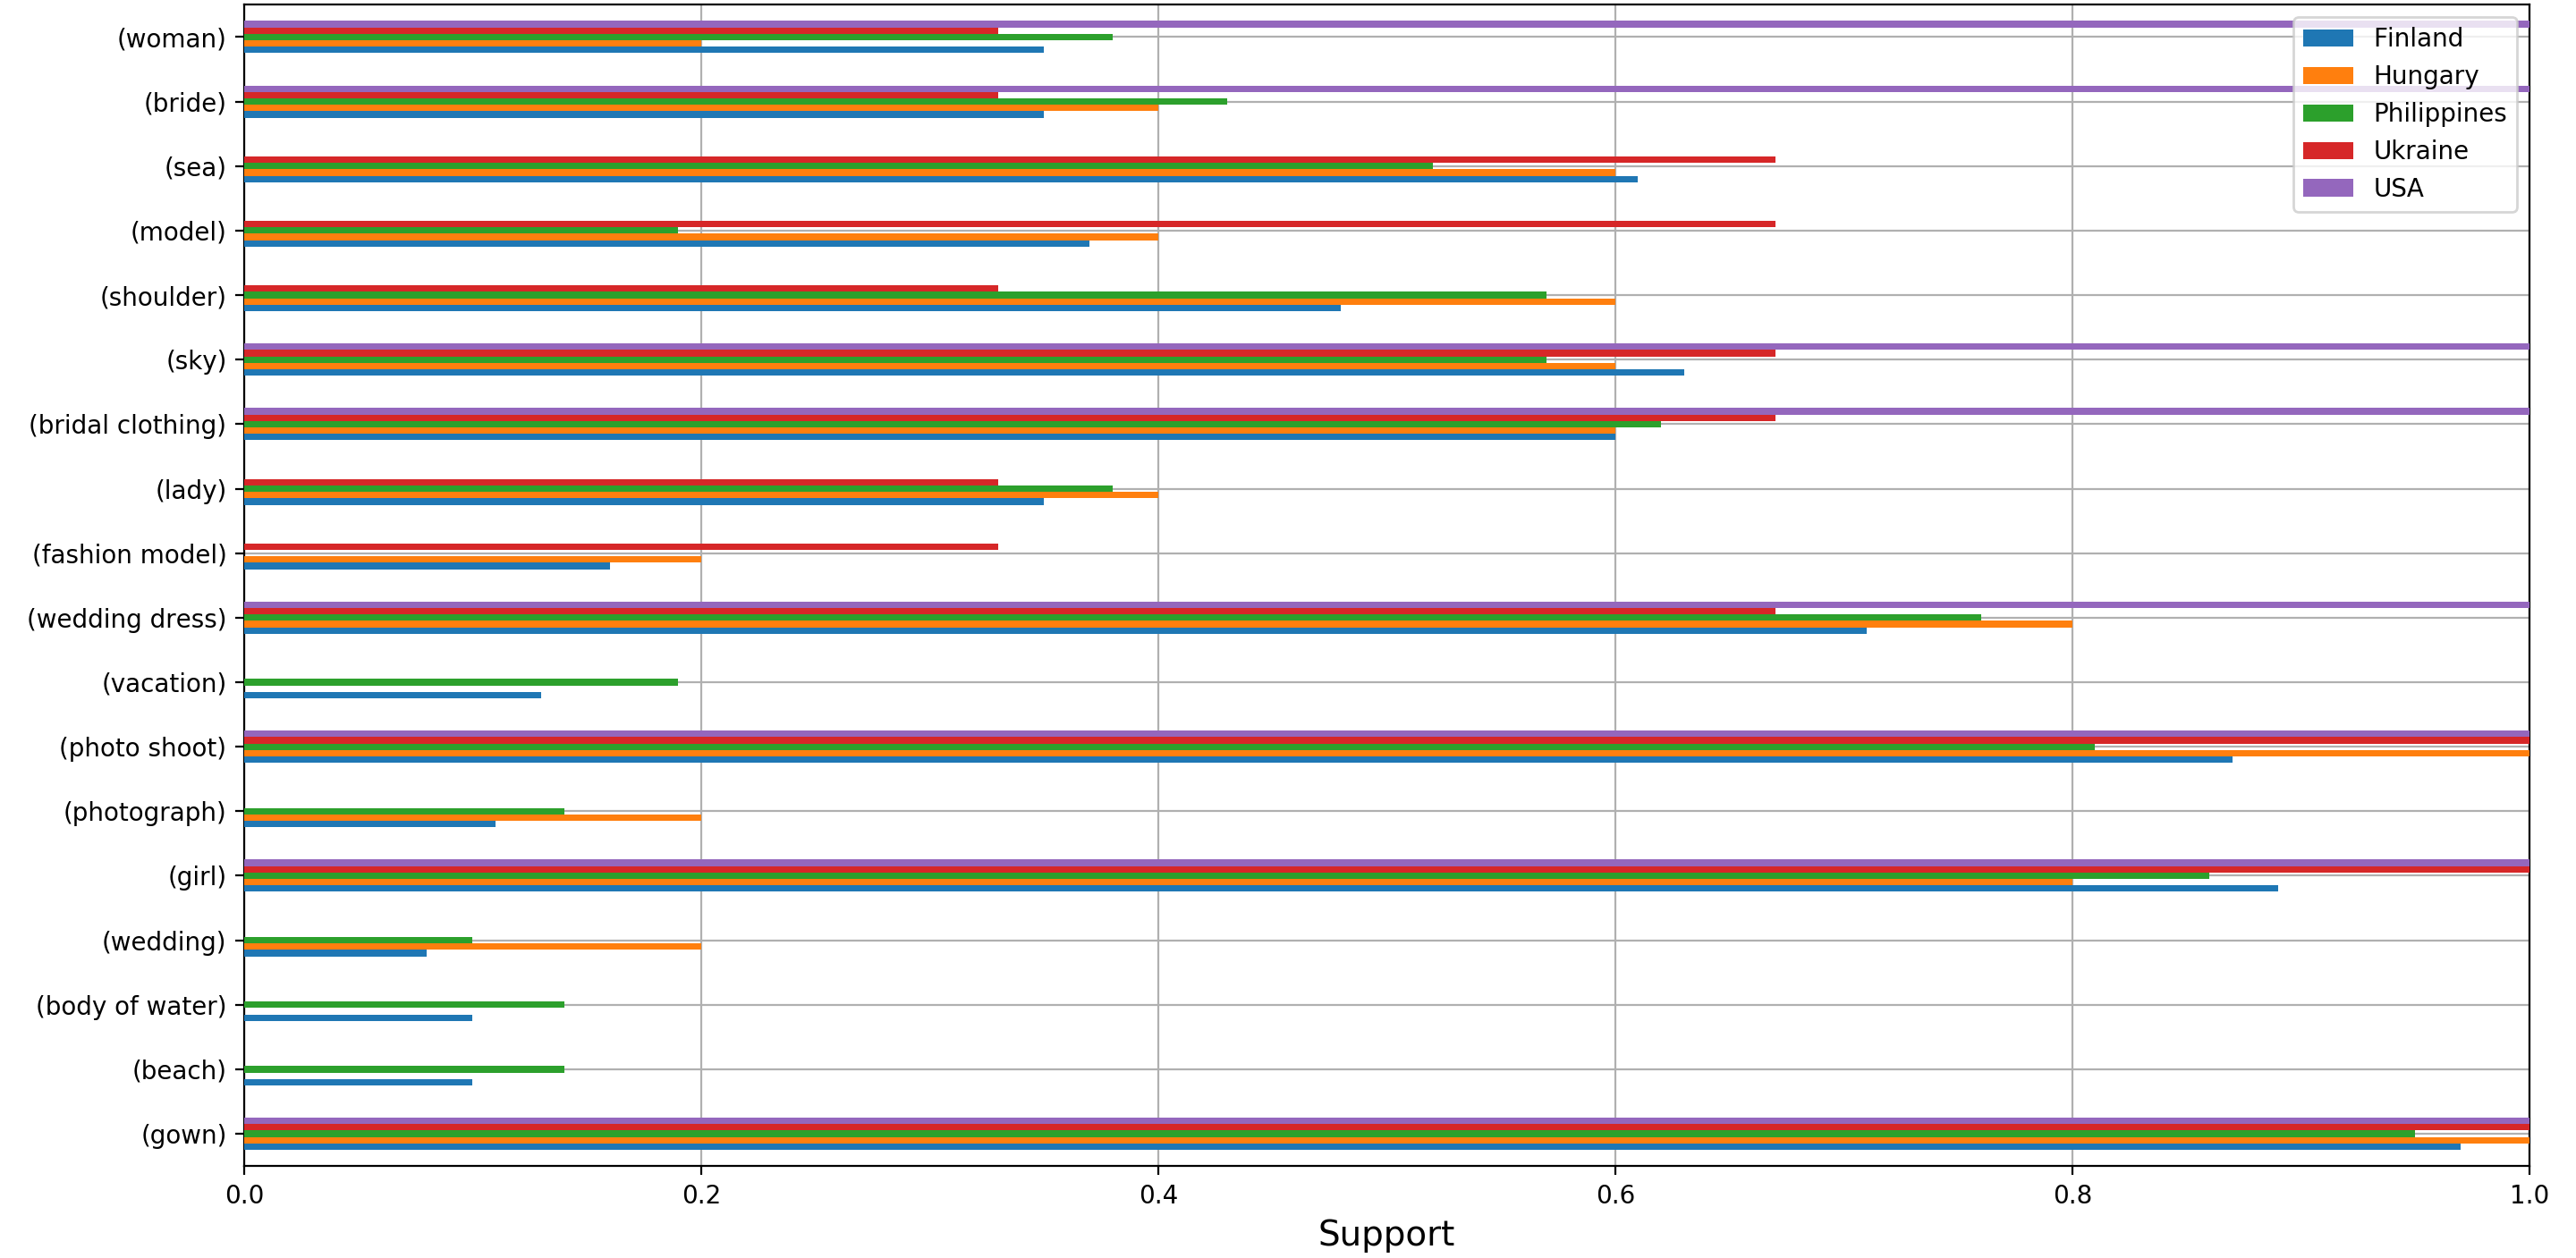
\includegraphics[width=1.2\textwidth,center]{Images/itemset_supports-country-Miss_Helsinki-1_itemset.png}
        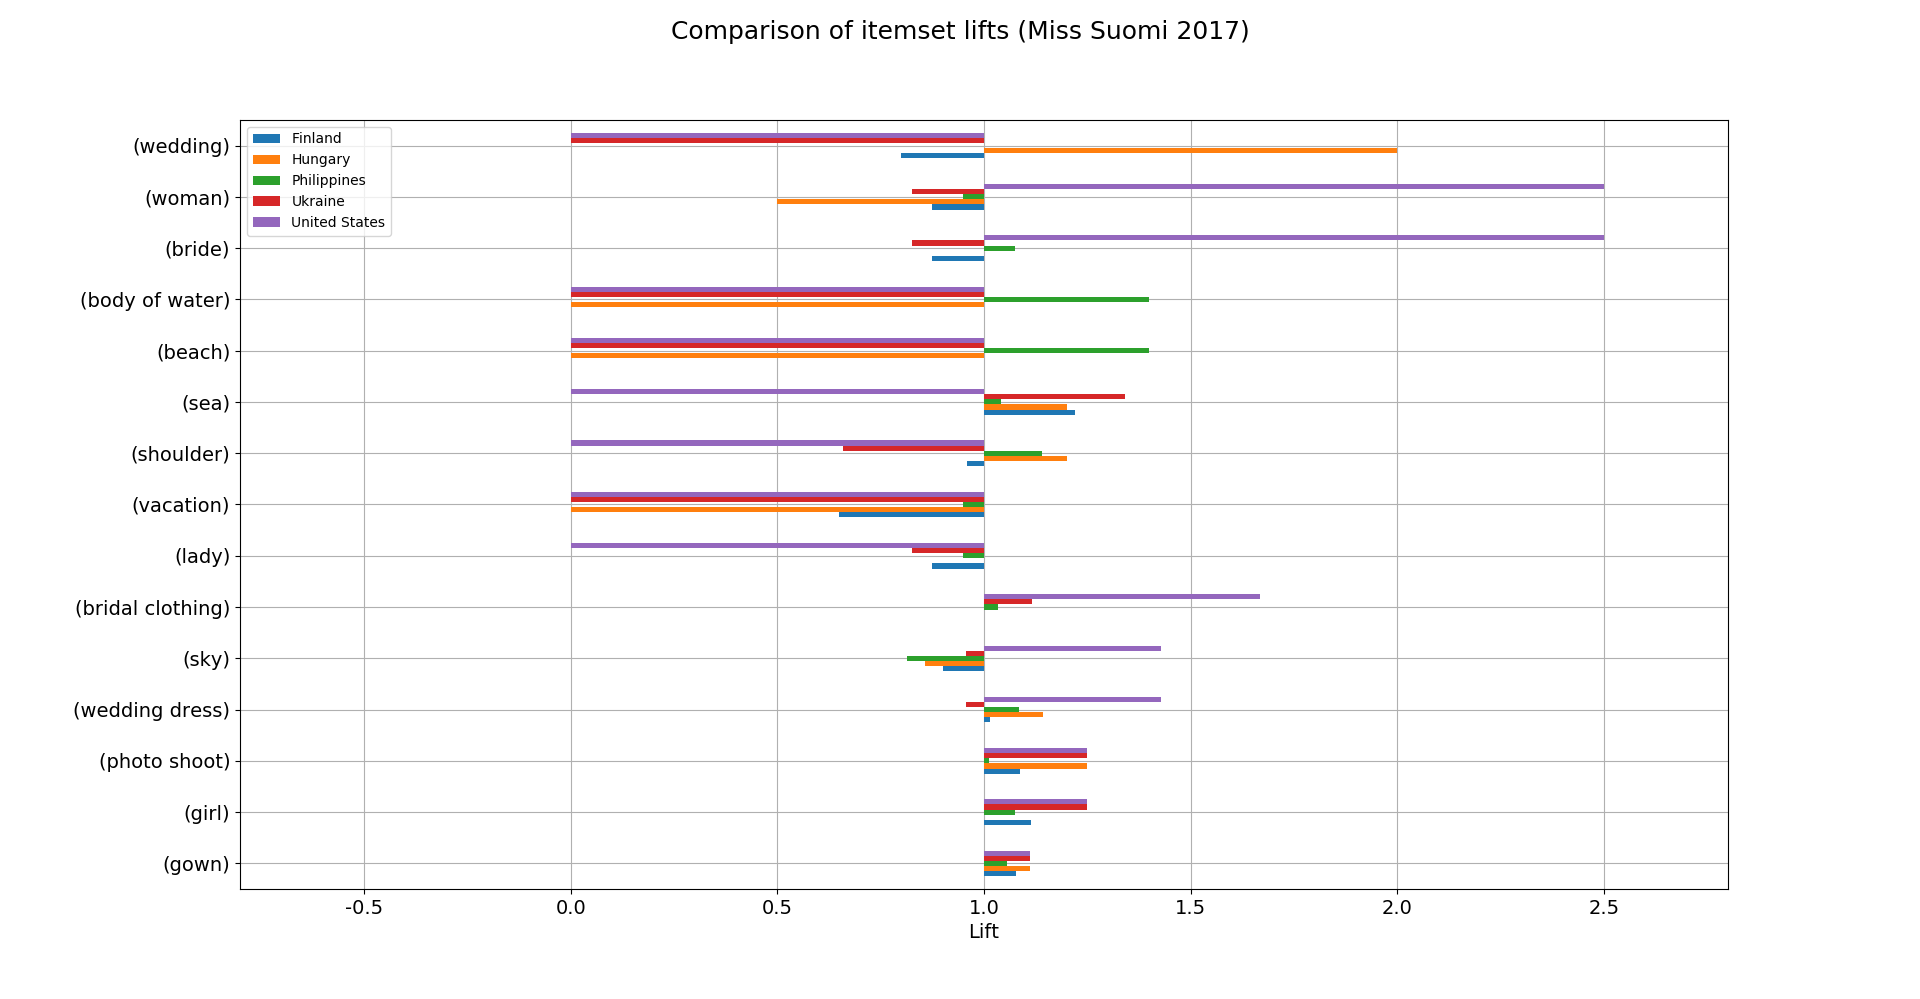
\includegraphics[width=1.2\textwidth,center]{Images/itemset_lifts-country-Miss_Suomi-1_itemsets.png}
        \caption{The 1-itemset supports (top) and lifts (bottom) in the Miss Suomi 2017 contest by countries.}
        \label{itemset_supports-country-Miss_Helsinki-1_itemset}
    \end{center}
\end{figure}

By looking at the data the reason becomes obvious: the amount of transactions, where the users' country information is set as USA, Ukraine and Hungary are considerably low (below 5). When looking at the lift values this bias comes even more appealing for users in USA and Ukraine. This may not be a big surprise knowing that this contest was mainly advertised in Finland and not in other countries. As a matter of fact, there were 62 Finnish voters and 21 voters from the Philippines, which are still considerably low compared to the total number of voters. 

This finding suggests that many of the voters in this contest did not indicate their country information and hence do not display on Figure \ref{itemset_supports-country-Miss_Helsinki-1_itemset}. In other words, the amount of users, whose location information is filled is too low. Hence, the results of these groups are only the upper and lower extremes, which means bias in the data. It can be also said that this particular contest did not engage users across borders on a broad scale and therefore is not a good case for this kind of analysis.

Encouraging the users in the future to provide more information would allow to derive valid results. At the present time, no strong conclusions can be drawn from the location data of the voters in the Miss Suomi 2017 contest. To ensure the relevance of the support and lift calculations, it would be hence a good move to put a lower limit (e.g. 100 observations) on the number of voters, similarly as it was done in the EDA phase for number of unique voters in contests. For all of the above reasons, no more analysis on the country-based support and lift values is performed in the remainder of this study.

% ---------------------------- END OF COUNTRY ANALYSIS ---------------------------- 
% ---------------------------- BEGIN OF 2-ITEMSETS ---------------------------- 
\pagebreak
% \subsubsection{Multi-item itemsets}

The next step of the Association Analysis covers the investigation on k-itemsets, where the \emph{k}-value is higher than 1. Figure \ref{itemset_supports-gender-Miss_Helsinki-2_itemset} displays the support values for the 2-itemsets by genders. To enhance the readability of the figure, only the first 15 values are shown. 

\begin{figure}[h] 
    \begin{center}
        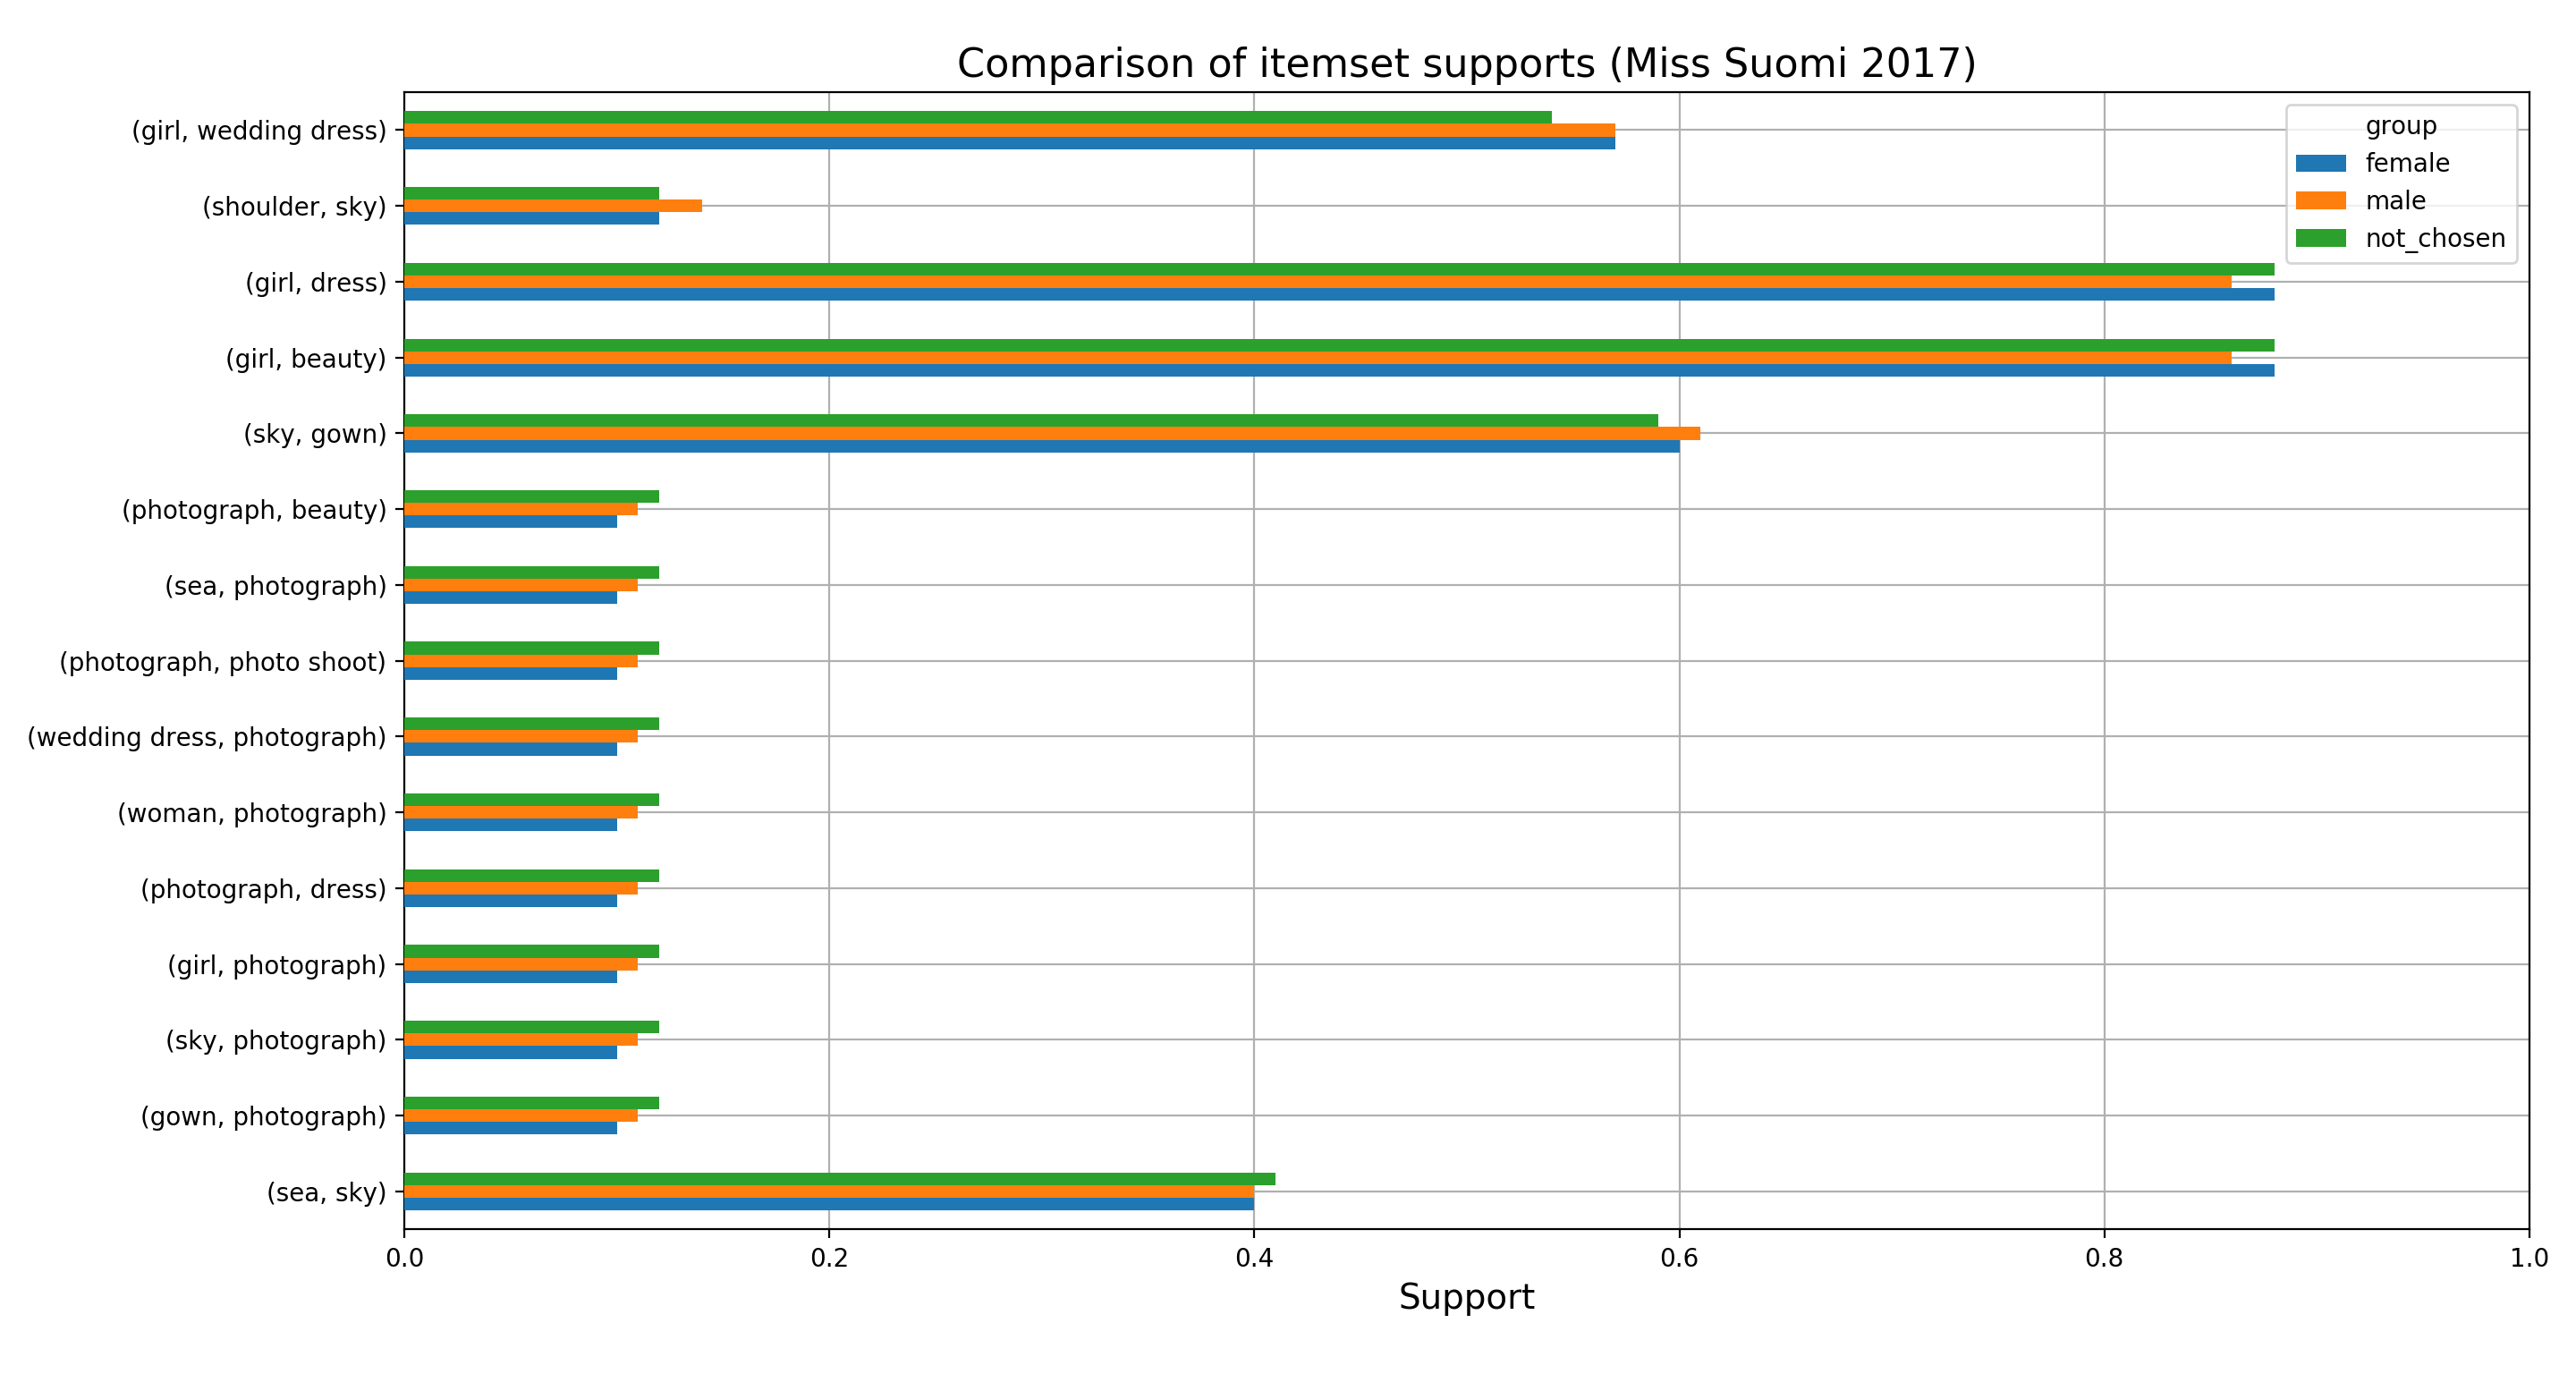
\includegraphics[width=1.2\textwidth,center]{Images/itemset_supports-gender-Miss_Helsinki-2_itemset.png}
        \caption{The 2-itemset supports in the Miss Suomi 2017 contest by genders (only the first 15 itemsets are displayed, ordered by variance).}
        \label{itemset_supports-gender-Miss_Helsinki-2_itemset}
    \end{center}
\end{figure}

% closed frequent itemsets
An important observation to make is the identicality of the 2-itemsets, where \emph{"photograph"} is present. This is due to the fact that all of the pairing itemset \emph{Y} (i.e. \emph{\{"beauty"\}, \{"sea"\}, \{"photo shoot"\}} etc.) are always present on images, where \emph{"photograph"} is present. In other words, the confidence \emph{C("photograph"|Y) = 1.0}, where \emph{Y} is the itemset next to \emph{"photograph"}. This is known as a Closed Frequent Itemset phenomena \cite{introtodatamining}. Closed, because the data contains no superset that has the same support value as this original itemset and frequent, because the itemset's support exceeds the \emph{minsup} threshold \cite{introtodatamining}. For this reason, when discussing 2-itemsets, this issue may arise and provide identical support values for some combinations. When the complete list of 2-itemsets is plotted, the same observation can be made for many other itemsets, such as \emph{\{"bride"\}}, \emph{\{"shoulder"\}}, \emph{\{"body of water"\}}, etc. 

% address the problem of closed itemsets
To address this issue, such closed itemsets are merged and analyzed together. In the above example (Figure \ref{itemset_supports-gender-Miss_Helsinki-2_itemset}, itemsets with \emph{\{"photograph"\}}), the identical 2-itemsets are merged into a single itemset, such that it contains \emph{\{"photograph", "beauty", "photo shoot", "gown", ..., "woman"\}}. This way the combined itemset has 10 items in overall. This is done repeatedly for all Closed Frequent 2-itemsets. The support and the lift values are then calculated for the resulting itemsets. For the sake of similicity and interestingness, the support values are not displayed here. Figure \ref{itemset_lifts-gender-Miss_Suomi-multi_itemsets} displays the lift values for genders. Similar results for age groups are listed in the appendices but are not analyzed in the paragraphs to follow.

\begin{figure}[]
    \begin{center}
        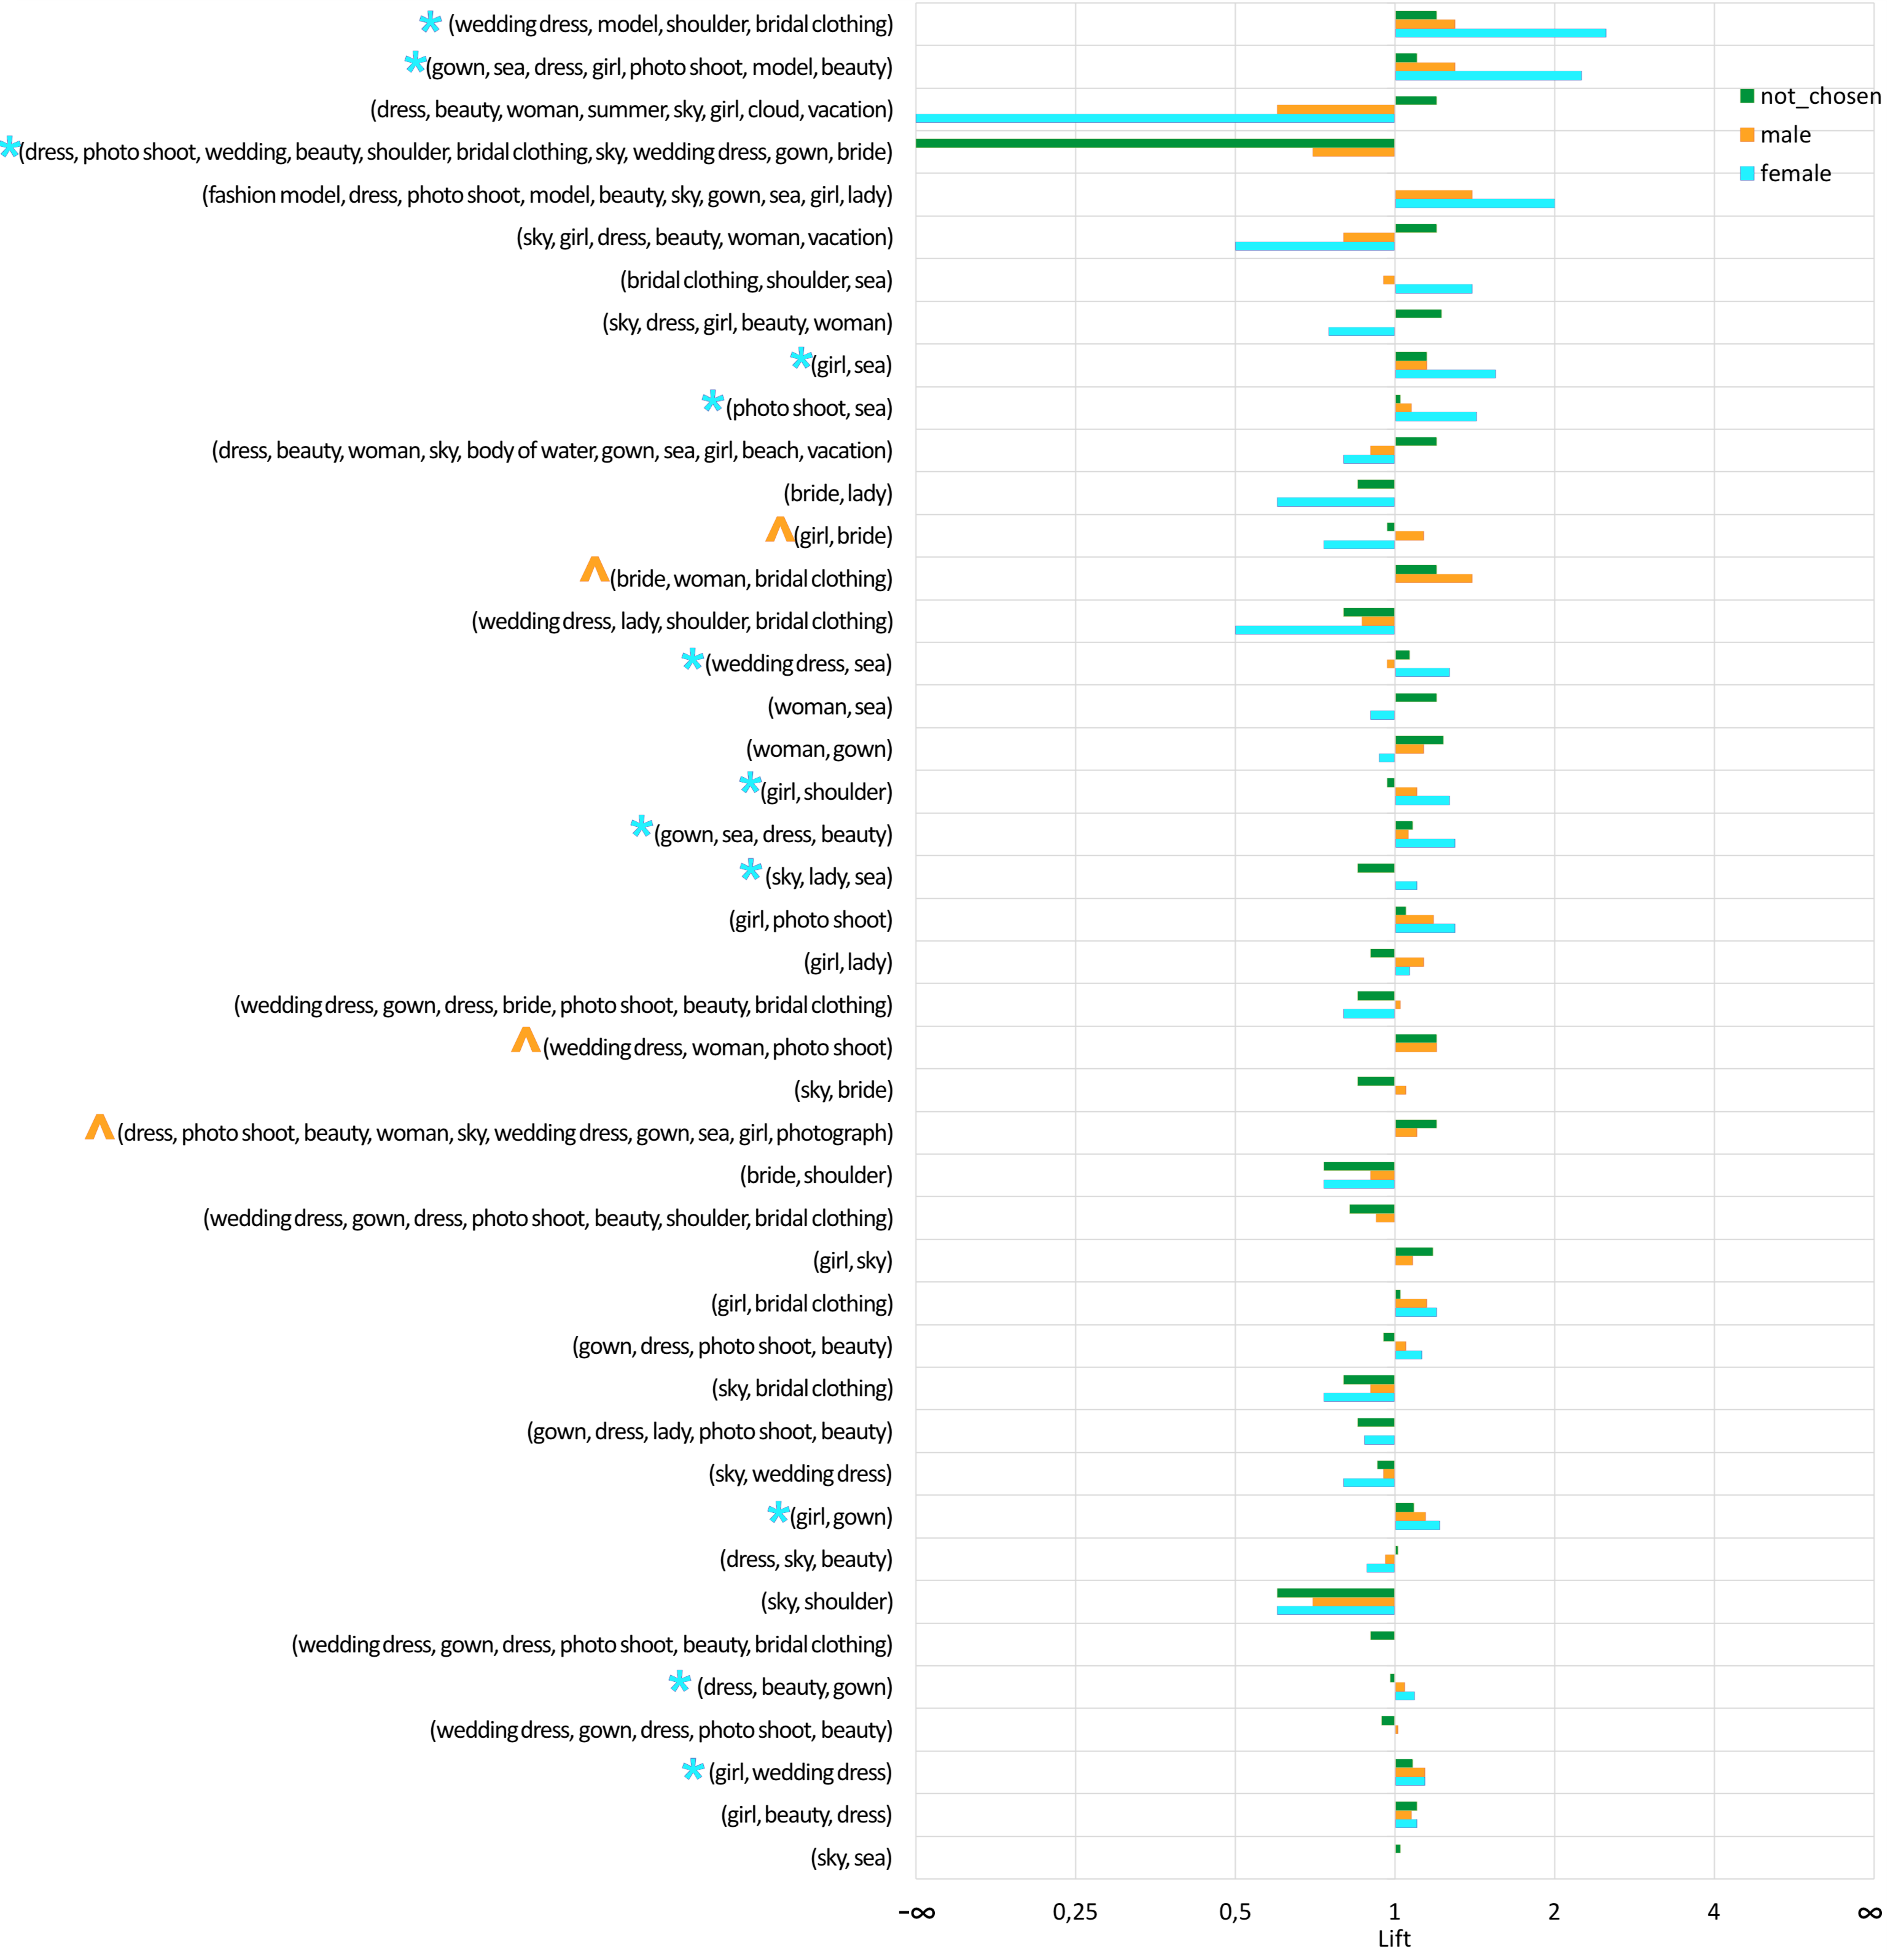
\includegraphics[width=1.2\textwidth,center]{Images/itemset_lifts-gender-Miss_Suomi-multi_itemsets+markup.png}
        \caption{The multi-item itemset lifts in the Miss Suomi 2017 contest by genders (all itemsets are displayed ordered by the variance of the values).}
        \label{itemset_lifts-gender-Miss_Suomi-multi_itemsets}
    \end{center}
\end{figure}

The results show that the lift values for females tend to be higher than the other groups in many cases. These suggests high interest towards the topics that appear in the itemsets compared to the rest of the groups. Such itemsets are marked with a blue * mark on the left side of the figure. As the number of items in the itemsets varies, these often share similarities, but they also describe certain topics. For instance, it can be seen that the items in the sets are telling about a lady wearing some sort of wedding/bridal dress. In other words, the items which explain the dress as such are more dominant and appear accross multiple itemsets. 

Other itemsets show more attraction from male voters. These are marked with an orange \^ on the left side of the figure. In contrast, these itemsets describe not the dress as much as the model on the image and the background (sea, sky). It can be hence speculated that female voters might relate to the dress and the model (maybe think about themselves as being the models wearing the dress), while male voters might focus on the setting and the model in the image more.

Another interesting observation is that male voters' lift rarely goes to extremes, but usually is around the value of 1.0 in most cases. In contrast, the lift for the female group goes to extremes in both end for many more itemsets. This may suggest that females follow more of a specialist approach than males, who are more generalists. Based on these results it seems, that females are strongly engaged towards certain topics in this contest while males are engaged accross multiple topics which appear in the contestants' images.

% Another observation to be made on Figure \ref{itemset_supports-gender-Miss_Helsinki-2_itemset} is the behavior of the 1-itemsets, which had support of 1.0 on their own (\emph{\{"beauty"\}} and \emph{\{"dress"\}}, Figure \ref{itemset_supports-gender-Miss_Helsinki-1_itemset}). When these itemsets are paired with other itemsets, the support of the union is guaranteed to be the support of the set alongside. This implies also that any 1-itemset combined together with such itemsets has no impact on the support value. Therefore, 2-itemsets which include such label (that appears on all of the images) are non-informative and should be hidden. Another possibility is to study the lift instead of the support value, which in such cases can tell more about the value of such combinations.

% There is a total number of 150 2-itemsets in the image labels of the Miss Suomi contest, which is hard to analyze for the human eye. This number grows further with number of items in the set. To tackle this problem, itemsets with more than 1 item are not investigated the same way. Instead, the Co-Clustering approach is applied on the data to identify itemsets, that appear similar to eachother in their support. The details on this analysis and the results are explained in the next chapter. 

% ---------------------------- BEGIN OF SYSTEM-LEVEL ---------------------------- 
The final part of the Association Analysis has taken a look at itemset supports and lifts on the system level. That is, all of the vote transactions from contests with 100 unique voters were extracted from the system. This is the same dataset, which was used for the major part of the EDA in Chapter \ref{section::exploratory-data-analysis}, containing a total of 166808 votes over 81 contests. 

The biases in the data become appearent when the votes are studied on the system level. Most of the itemsets reflect on the great majority of "beauty" and "fashion" category contests, as itemsets such as \emph{\{"model"\}, \{"beauty"\}, \{"photo shoot"\}, \{"shoulder"\}} etc. From the itemset supports it seems that all of the itemsets were extracted from contests of these two category, as they clearly describe concepts that appear in such contests. This observation also supports the previous finding, that mainly contests in these categories were hosted in the platform with great success.

While studying the results it was identified, that the \emph{not\_chosen} group has considerably higher support over males and females in many cases. This can be explained by the fact that many users (49.82 \%) did not provide their gender information on their profile, which yields in a much higher number of observations (vote transactions) for users whose gender is unknown. 46.4 \% (77416 observations) from the the vote transactions were received from users with unknown gender. Likewise, only 27 \% (44918 observations) of the votes were received from females and 26.6 \% (44407 observations) from males. Similar observations can be made for the age group values, where 67 \% of the voters have not filled their age. 

It can be therefore seen that the sample size of the \emph{not\_chosen} gender and age group is dominant in the system-wide data. This creates a bias in the support values as the data for these group is more representative than for others. While this problem did not emerge on a single-contest level, when looking at all transactions, it becomes apparent. It could be assumed, that the distribution of the two genders is equal in this group, however there is no proof on this claim. For these reasons, strong claims and concrete findings are harder to derive from this data due to the bias explained above. The system-level data is therefore not analyzed, however some of the extracted figures are displayed in the appendices. 

\subsection{Co-Clustering}
The chosen Co-Clustering algorithm (Chapter \ref{section::methodology}) first was executed on a smaller set of 2-itemsets in the Miss Suomi 2017 contest. In this analysis, the \emph{minsup} value was set to 0.4 to focus only on the itemsets with higher support. This was done in order to first understand and demonstrate how the algorithm works in a smaller scale, similarly as it was done in the previous chapters. Then the method was applied on the Miss Suomi 2017 contest as well as on the system level for all itemset sizes in both cases with the \emph{minsup} value of 0.05. Various number of clusters was tried out with various observations depending on the dataset size and the demographic groups being analyzed. The results are explained in the paragraphs to follow. 

First, a smaller set of itemsets in the Miss Suomi 2017 are chosen for a more careful analysis. The filtering by support here is done by first collecting the support values of the 2-itemsets for genders and age groups (same way it was done during the Association Analysis, shown on Figure \ref{itemset_supports-gender-Miss_Helsinki-2_itemset}). Then all of the itemsets were dropped, where the highest value did not exceed the $0.4$ \emph{minsup} threshold. This way 54 instances of 2-itemsets remain in the dataset.

Next, the matrix of the itemsets is plotted on the left side of Figure \ref{coclustering_miss-suomi-genders-2-itemsets-04_support}. The colors correspond to the support of the itemset: the lighter values indicate smaller, the darker blue colors indicate higher support values. It can be seen that for instance the \emph{\{"dress", "beauty"\}} has high, while the \emph{\{"sky", "sea"\}} considerably low support among the demographic groups. The left side of the figure is not organized in any way, hence there is no pattern in how the colors appear in the chart. 

\begin{figure}[] 
    \begin{center}
        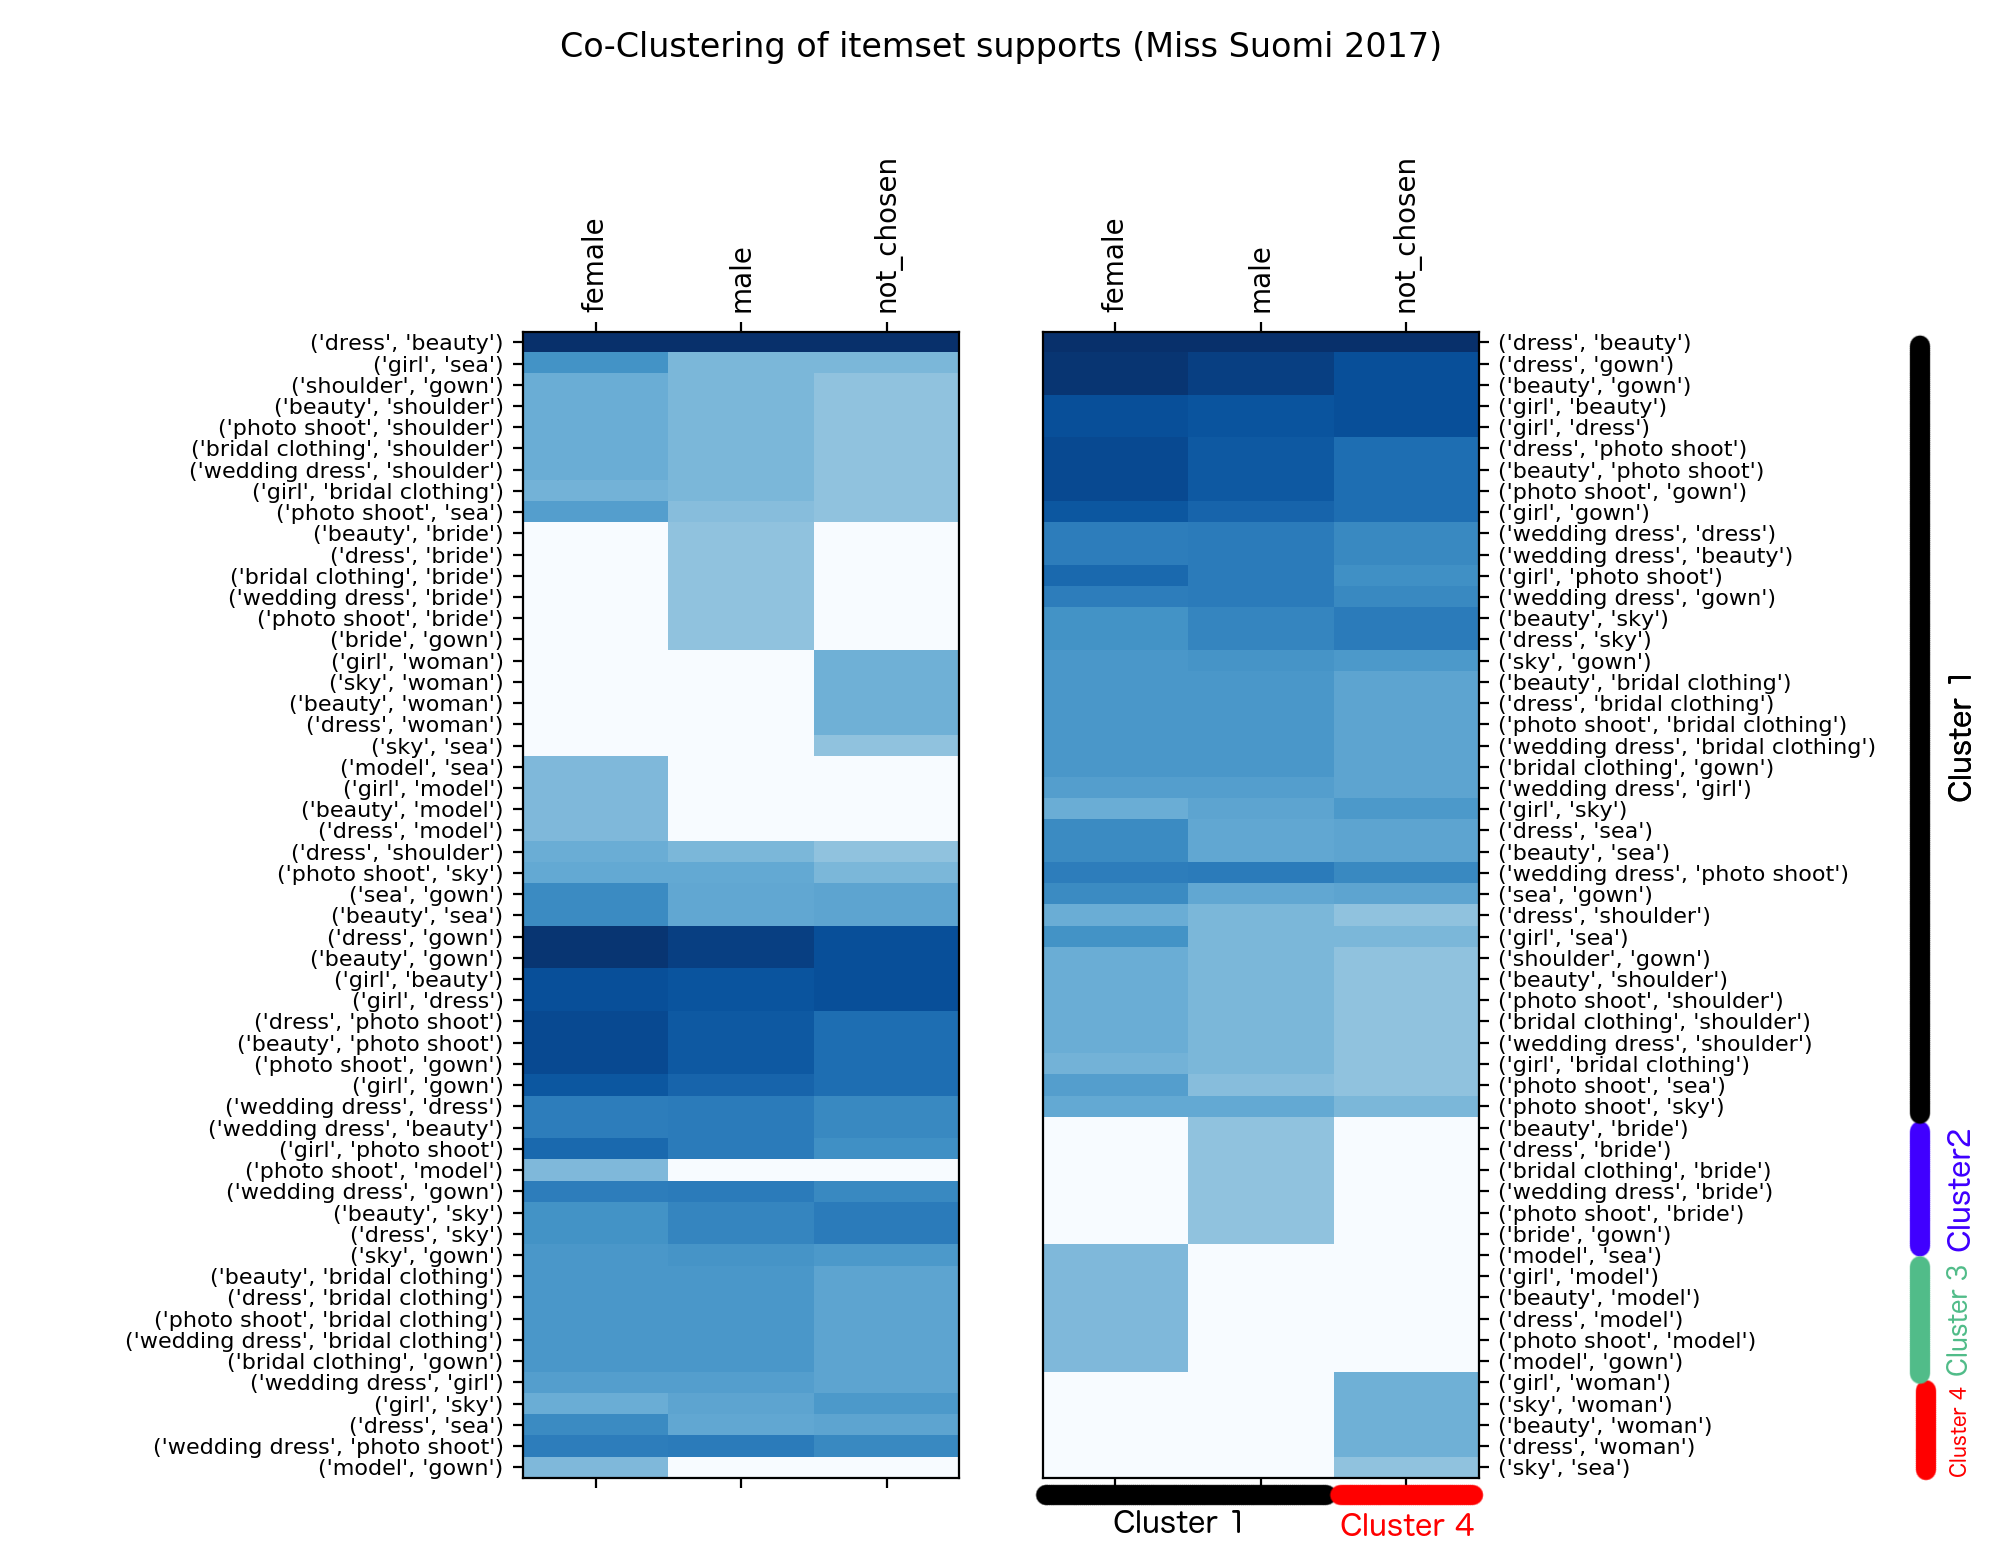
\includegraphics[width=1.2\textwidth,center]{Images/coclustering_miss-suomi-genders-2-itemsets-04_support.png}
        \caption{The results of the Co-Clustering in the Miss Suomi 2017 contest for 2-itemsets over 0.4 support with 4 clusters by genders. Left: the itemsets before clustering; Right: the itemsets after clustering.}
        \label{coclustering_miss-suomi-genders-2-itemsets-04_support}
    \end{center}
\end{figure}

The right side of Figure \ref{coclustering_miss-suomi-genders-2-itemsets-04_support} dislays the result of the Co-Clustering algorithm with 4 clusters. The markups on the side and the bottom of the chart indicate the clusters to which the rows and columns were assigned. Choosing the number of clusters was essentialy done by looking at the results and analyzing which k-value produces the most sensible results in this particular case. 

It can be seen that males and females were assigned to the same cluster in this case (cluster 1) with most of the itemsets that have higher support values. This finding suggests that there are no significant differences between males and females in this case. Interestingly, the algorithm has put the "not\_chosen" group to its own cluster (cluster 4) with only a few itemsets. This result may suggest that this group is significantly different than the other two, even though it can be seen that the supports in cluster 1 are also considerably high. 

If clusters are looked at from the aspect of the itemsets, it can be concluded which ones seem to belong together. For instance, clusters 2 and 3 clearly pinpoint the itemsets that engaged only males and females respectively in this case. This can be another useful information to marketers, whose aim is to target one of these groups with certain content. Another useful aspect in this visualization is, that the itemsets with various supports can be distinguished easily based on the color's depth. Identifying itemsets that belong together is considerably easier on the right side of the figure as the Co-Clustering algorithm puts these close to eachother. 

Figure \ref{coclustering_miss-suomi-age_group-2-itemsets-04_support} displays the results of the same analysis for age groups. When filtering the data this way, the amount of 2-itemsets rises to 76. As there are more transactions and demographic groups, the number of clusters was increased to 5 on this occasion. 

\begin{figure}[] 
    \begin{center}
        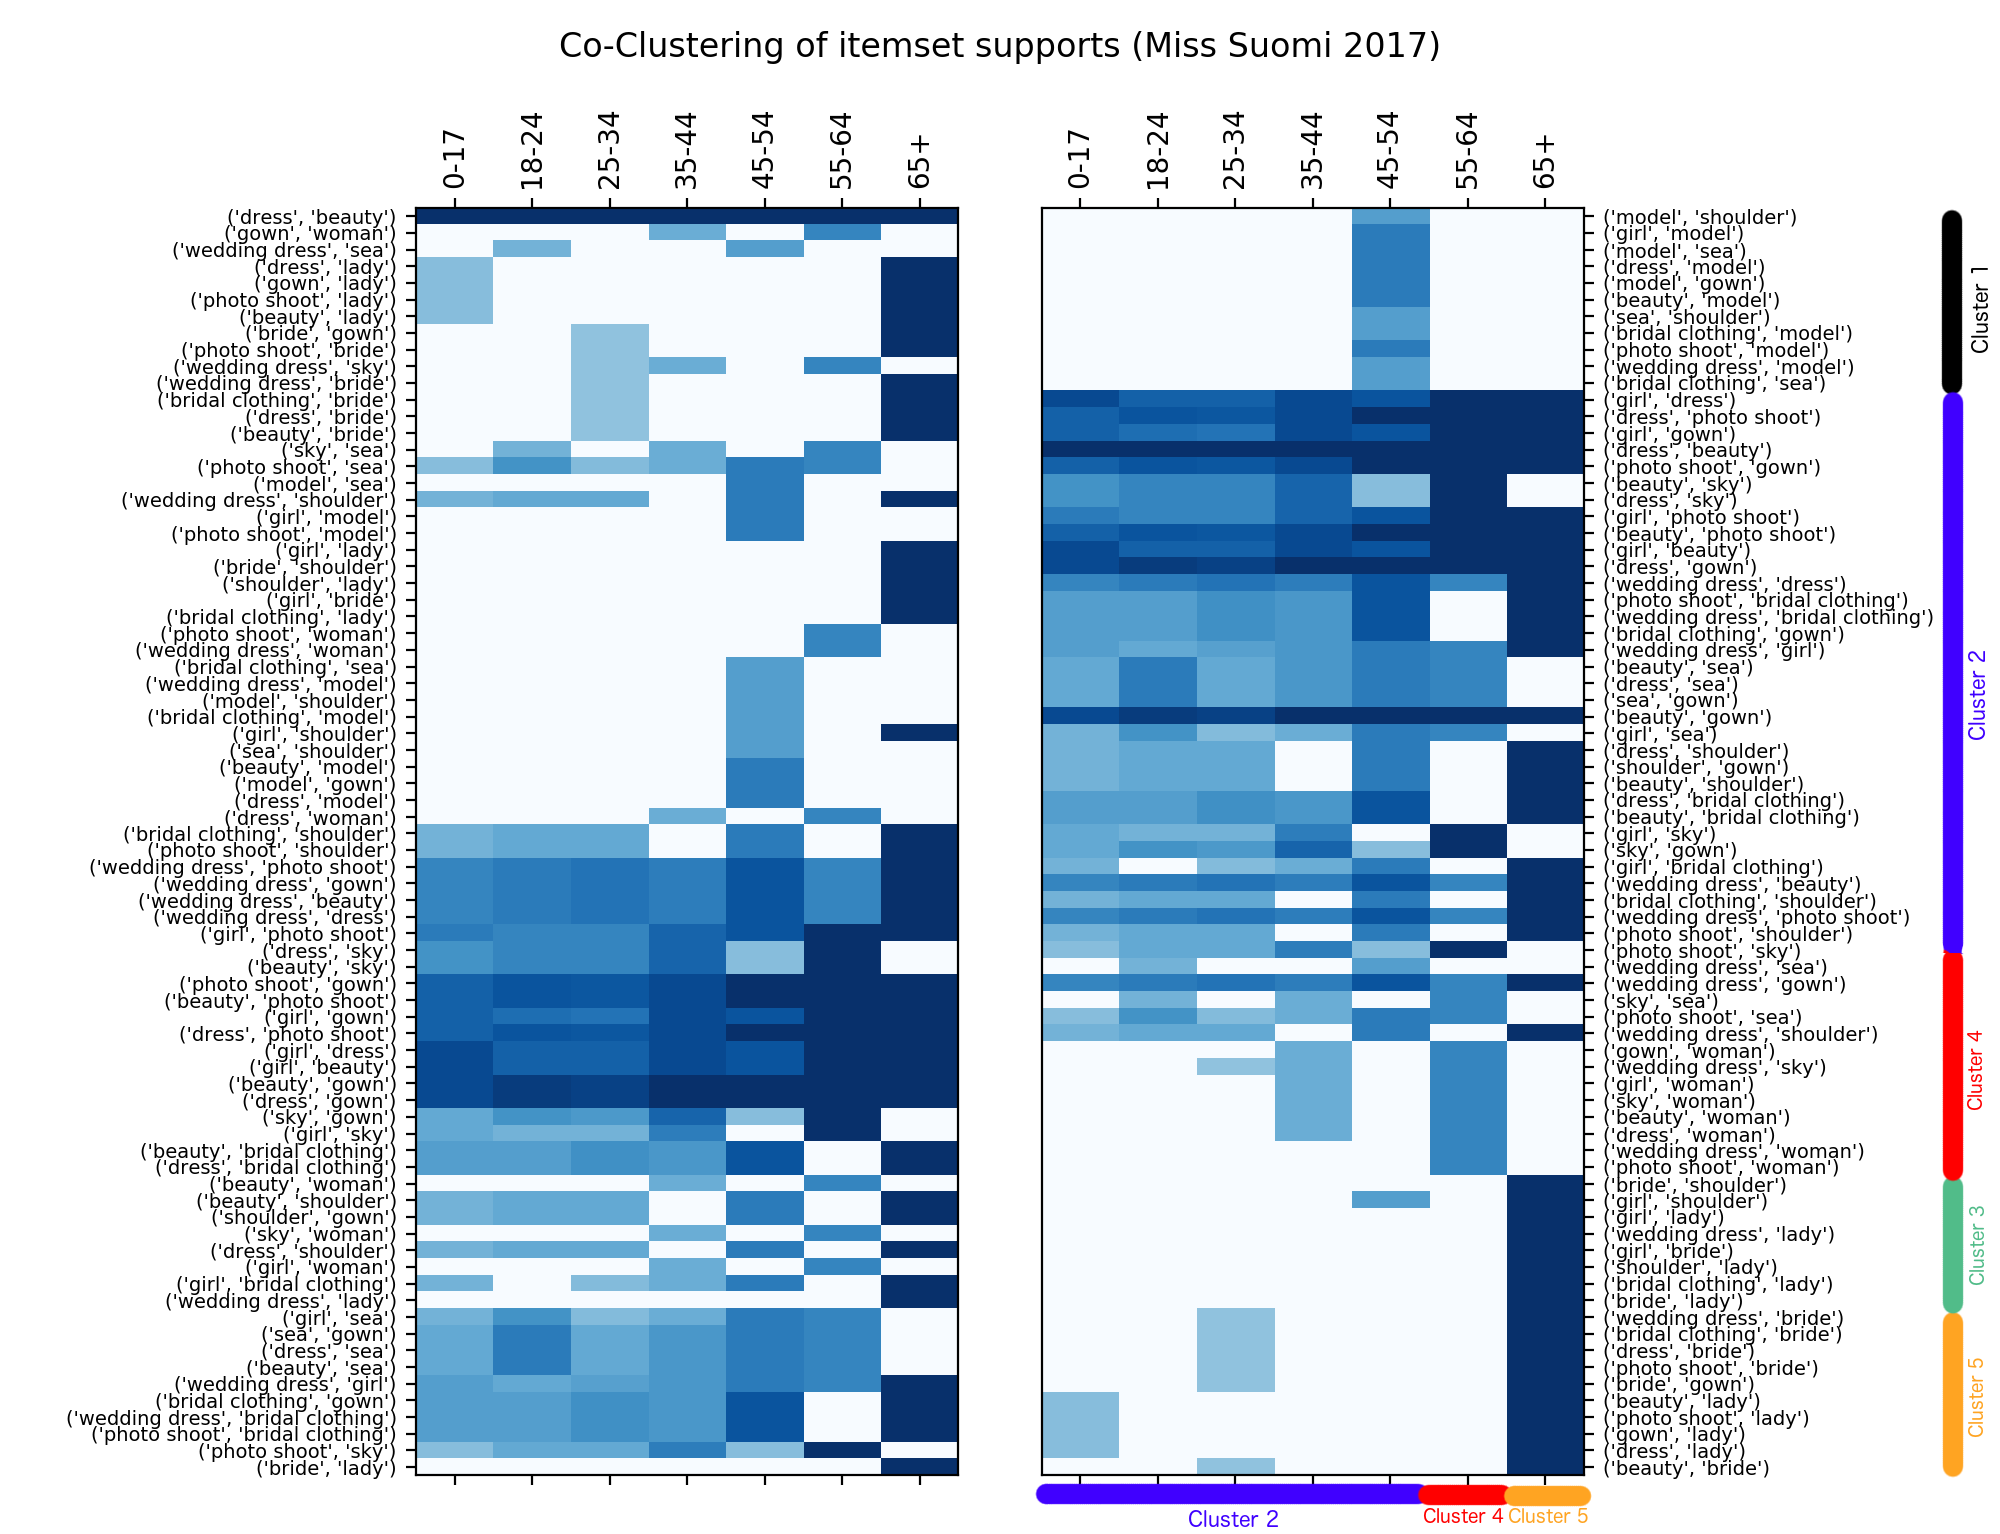
\includegraphics[width=1.2\textwidth,center]{Images/coclustering_miss-suomi-age_group-2-itemsets-04_support.png}
        \caption{The results of the Co-Clustering in the Miss Suomi 2017 contest for 2-itemsets over 0.4 support with 5 clusters by age groups. Left: the itemsets before clustering; Right: the itemsets after clustering.}
        \label{coclustering_miss-suomi-age_group-2-itemsets-04_support}
    \end{center}
\end{figure}

One of the most interesting observations in this case is that the age groups 45-54 and 65+ are separated from the rest of the groups. This indicates that the interests of these groups are somewhat unique compared to the others. This finding is supported by the fact that itemsets in clusters 3, 4 and 5 have higher support from one a subset of the groups. However, cluster 2 contains most of the itemsets that are supported by all of the groups. The rest of the age groups are also assigned under cluster 2, which suggests the generality of these itemsets and groups. 

It could be hence concluded, that some demographic groups follow a generalist, some others a specialist approach. In this particular case, users between the age of 0-54 are more specialists towards the itemsets in cluster 2. Likewise, users from groups 55-64 and 65+ are unique, because some content (in clusters 3, 4 and 5) is engaging only to them. As a conclusion, they could be called as generalists. This finding is in align with the results of Jang et al. \cite{jang2015no}, who also identified similar findings on social media. 

Finally, the Co-Clustering is executed on the system level. The \emph{minsup} value is set to $0.05$ for this analysis and the itemset size is not limited to any numbers. When performing the analysis for genders, the same observation can be made as during the Association Analysis, namely that the \emph{not\_chosen} group creates a bias in the data, because this group has higher support values for most itemsets. Inevitably, this fact also has an impact on the behavior of the Co-Clustering algorithm. 

With 4 clusters and $166 808$ vote transactions, the results are as follows. All three genders (male, female and not chosen) are assigned to their own clusters with a subset of the itemsets in the platform. This findings suggests that the different genders tend to behave differently on the system level and there is a difference in which itemsets engage them. 

The majority of the itemsets ($977$ out of $1 626$) are assigned to the "not\_chosen" group, which is the consequence of the observation stated in the previous paragraph. Interestingly, the number of itemsets for females ($148$) is considerably lower than for males ($482$). This suggests that males have wider range of interests than females, if the data is analyzed on the system-wide level. There are $19$ itemsets that are not assigned into the same cluster with any of the demographic groups, which may mean that these are on the same level of interest for all of the groups. 

When the system-wide analysis is performed for age groups with the same settings, the results are as follows. Similarly to genders, the users whose age is unknown are grouped under their own specific cluster with most of the itemsets ($888$ out of $2 332$). However, it is interesting to observe that age groups 0-17, 18-24, 25-34 and 45-54 are grouped under the same cluster with $314$ itemsets. Age group 35-44 has its own cluster with $578$ items and the 55-65 and 65+ age groups are again clustered together with $551$ itemsets. 

It can be seen that there is a clear distinction between the younger and the older generation in the clustering. This finding suggests that the engaging content is different for these groups, while the middle-aged (34-54) users are somehow between them. The algorithm was executed with various number of clusters, but this behavior was always present. This observation further enhances the validity of this finding and suggests further investigation on the reasons in this area.

% how is this all going to be used/integrated into the platform?
% \subsection{Implications}